%%%%%%%%%%%%%%%%%%%%%%%%%%%%%%%%%%%%%%%%%%%%%%%%%%%%%%%%%%
%   Autoren des Abschnitts:
%   Jakob Kautz
%   Olivier Stenzel
%%%%%%%%%%%%%%%%%%%%%%%%%%%%%%%%%%%%%%%%%%%%%%%%%%%%%%%%%%

% !TEX root =  master.tex
\graphicspath{ {./img/} }

\chapter{Konzeption - Hardware}\label{konzeptionHW}
\chapterauthor{Jakob Kautz, Olivier Stenzel}

% @TODO(Val): Erst erklären warum MCs und Aktuatoren benötigt werden, bevor erzählt wird, dass wir die irgendwie verwenden müssen. Sonst argumentieren wir mit technischer Lösung statt dem Problem. Wenn wir die Erklärung dafür erst später haben wollen, sollten wir hier zumindest anfangs schon erwähnen, dass wir später noch erklären, warum Aktuatoren und ein MC benötigt werden oder so

Für die Umsetzung eines selbstspielenden Klaviers wurden verschiedene technische Überlegungen angestellt.
Die Grundfragen, welche bei der Konstruktion auftreten, betreffen die Methode des Anspielens der Klaviertasten, die
Signalübertragung des \ac{MC}s, sowie die Konzeption der Schaltung.
Folgende Anforderungen muss die Konzeption abdecken:


\begin{enumerate}
	\item \textbf{Ansteuerungskonzept:} Die Tasten müssen möglichst präzise und effizient von der Hardware angespielt werden können; dies beinhaltet Positionierung der Aktuatoren und die Verbindung zwischen Hardware und Klavier
	\item \textbf{Auswahl der Aktuatoren:} Die Aktuatoren müssen eine präzise Steuerung der Tasten ermöglichen, ohne dass Genauigkeit und Geschwindigkeit des Anspielens der Tasten vernachlässigt wird
	\item \textbf{Auswahl des \ac{MC}:} Die Aktuatoren benötigen zur Ansteuerung der Klaviertasten die Signale der Software, wobei die Kommunikation über einen \ac{MC} geschieht
\end{enumerate}

Die Überlegungen und Entscheidungen für die genutzte Hardware sowie den Aufbau dieser werden in diesem Kapitel erläutert.
Die Hardware-Komponente des Projektes wird im folgenden auch als \enquote{Piano Player} bezeichnet.

\section{Mechanik}\label{konzeptionHW-mechanik}

\subsection{Auswahl des Klaviers}

\chapterauthor{Olivier Stenzel}

Da sich dieses Projekt nicht auf die theoretische Konzeption beschränkt, muss ein entsprechendes Testobjekt - ein reales Klavier - gefunden werden.
Dieses muss einige Voraussetzungen erfüllen:
\begin{enumerate}
	\item 	Der Preis muss im Rahmen des selbst gestellten Budgets (< 2000\euro{}) liegen
	\item 	Es muss leicht auseinander zu bauen sein, damit die Mechanik zugänglich ist
	\item 	Es muss vollständig sein (alle 88 Tasten)
	\item 	Es muss stimmbar sein
	\item 	Der Transport muss einfach durchzuführen sein
\end{enumerate}

Mittels dieser Anforderungen wurde online ein passendes Klavier für 100\euro{} ersteigert.

\subsection{Ansteuerungskonzept} \label{subsec:konzeptionhw-ansteuerungskonzept}

\chapterauthor{Jakob Kautz}

Das Ansteuerungskonzept bezieht sich auf die Problemstellung, dass die Saiten des Klaviers auf irgendeine Art automatisiert zum Schwingen gebracht werden müssen.
Dafür ist eine Vorrichtung hilfreich, die elektrische Signale in Bewegung umwandeln kann.
Dies ist die Eigenschaft von Aktuatoren, wie z.B. Motoren.
Ein Aktuator wandelt ganz genrell Energie in Bewegung (oder andere physikalische Größen) um, um eine gewünschte Aktion herbeizuführen oder einen Mechanismus zu steuern. \newline % @TODO(Val): Quelle für Aktuator-Definition

In diesem Kapitel wird untersucht, wie genau man das Anspielen der Saiten technisch umsetzen kann.
Dabei ist eine grundlegende Überlegung, ob man die Saiten direkt anschlägt,
oder die bestehenden Tasten dafür nutzt.

Wenn die Aktuatoren direkt die Saiten des Klaviers anspielen, erfordert dies weniger Kraft im Vergleich zum
Anspielen der Tasten. Das liegt daran, dass die Tasten eine größere mechanische Übersetzung bieten, um die Saiten
anzuschlagen. Wenn die Aktuatoren direkt auf die Saiten wirken, müssen sie nur die erforderliche Kraft aufbringen, um
die Saiten in Schwingung zu versetzen, was im Allgemeinen weniger Kraft erfordert als das Drücken einer Taste mit
ausreichend Kraft, um den Hammer gegen die Saiten zu schlagen.

Die Verwendung von weniger kraftaufwendigen Aktuatoren kann die Gesamtkosten des Systems senken. Aktuatoren, die weniger
Kraft erzeugen müssen, sind oft einfacher und kostengünstiger herzustellen (und zu kaufen) und erfordern möglicherweise weniger
energieintensive Komponenten. Darüber hinaus kann die Verwendung von leistungsschwächeren
Aktuatoren die Größe und das Gewicht des Systems verringern, was zusätzliche Vorteile hinsichtlich Kosten, Transport und
Montage bieten kann. \newline
Allerdings geht dabei die gesamte Mechanik des Klaviers verloren, was bedeutet, dass Aspekte wie Dämpfung nicht genutzt werden können,
was wiederum zu einem weniger ansprechenden Klang führt. Zusätzlich müsste das Klavier permanent geöffnet bleiben, und die
Aktuatoren müssten äußerst präzise die Saiten anschlagen, um akzeptable Ergebnisse zu erzielen.
Da die Erzeugung eines ansprechenden Klangs für dieses Projekt eine höhere Priorität annimmt, fiel die Entscheidung
darauf, die Tasten anzuspielen. Somit kann die Klaviermechanik genutzt werden, was für einen
authentischeren Klang sorgt. \newline
Nun stellt sich also noch die Frage, wie genau die Aktuatoren mit den Tasten des Klaviers verbunden werden.

Eine Möglichkeit besteht darin, die Aktuatoren oben über den Tasten anzubringen, entweder in Form einer nachgebildeten
\enquote{Klavierhand} mit zehn \enquote{Fingern} oder in Form einer Schiene mit 88 Aktuatoren auf den Tasten.
Beide Lösungen bringen allerdings das Problem mit sich, dass sie gegen die in Kapitel \ref{Zielstellung} definierte Anforderung A6
der Flexibilität verstoßen, nämlich dass das Klavier sowohl automatisch als auch manuell bespielbar sein soll.\newline
Außerdem würde die Klavierhand-Option - die dem tatsächlichen Klavierspiel ähnlich sieht -
aufgrund der Bewegung und Präzision eine komplexere Logik und
Montage erfordern. Die Schienenoption bietet hier eine viel einfachere Ansteuerung, benötigt jedoch einen Aktuator für jede Taste.
Außerdem steht diese Variante im Gegenspruch zur Anforderung A8, dass der Aufbau für unterschiedliche Klaviere anpassbar
sein soll. Das liegt daran, dass diese Schiene eine fest vorgegebene Länge hätte, welche für Klaviere mit anderen Größen nicht mehr passen würde. \newline

Eine Alternative hierzu besteht darin, die Aktuatoren unter den Tasten anzubringen, wodurch die Anforderung der Flexibilität nicht beeinflusst wird.\newline
Das Klavier kann also sowohl vom \enquote{Piano Player} als auch von einem menschlichen Spieler gleichzeitig bedient werden.
Da diese Anforderung eine hohe Priorität hat, wird die Ansteuerung von untern erfolgen. \newline
Grundsätzlich gibt es hierbei zwei Möglichkeiten für die Ansteuerung:
\begin{enumerate}
	\item Ziehen der Tasten
	\item Drücken der Tasten
\end{enumerate}
Bei beiden Varianten wird jede Taste mit einem Aktuator
ausgestattet, es werden also 88 Aktuatoren benötigt, was die Kosten % @Question(Jay) soll ich späteres Kapitel zu Kosten referenzieren oder so lassen?
im Gegensatz zu der von oben Spielenden \enquote{Klavierhand}
erhöht.
Generell ist die Drückoption ästhetisch ansprechender, da die Hardware sehr einfach versteckt werden könnte.
Somit würde die Illusion entstehen, dass die Tasten sich von alleine bewegen. Die Option erfordert jedoch eine hohe Präzision und könnte die
Tastenempfindlichkeit beeinträchtigen. Außerdem wäre aufgrund der präzisen Montage der Aktuatoren die Anforderung
der Anpassbarkeit (A8) aufwendiger zu erfüllen.

Für das Drücken der Tasten fallen noch weitere Probleme an. Um die Tasten drücken zu können, muss ein möglichst großer
Hebel aufgebracht werden, damit die Aktuatoren möglichst wenig Kraft für das anspielen aufbrauchen müssen.
Dieser Punkt ist besonders wichtig, wenn der \enquote{Piano Player} mit unterschiedlichen Lautstärken und Dynamiken spielen können soll (siehe Anforderung A10).
% @Question(Jay): Ist es offensichtlich dass das daran liegt dass wir dann auch leiser spielen können oder soll ich das noch erwähnen?
% @Answer(Val): Kruse findet das wahrscheinlich offensichtlich und wenn ich kurz drüber nachdenke komme ich auch drauf, aber wenn du das in einem Nebensatz kurz erwähnen könntest wäre es wahrscheinlich besser
Dies führt dazu, dass die Aktuatoren soweit hinten wie möglich angebracht werden müssen, um einen größeren Hebeleffekt zu erhalten.
\newline
Hierbei tritt nun das folgende Problem auf:
Der Holraum, der sich im hinteren Teil des ausgewählten Klaviers befindet, ist nicht durchgängig. Daher ist es
erforderlich, Löcher einzubauen. Diese müssen räumlich so platziert werden, dass sie keine wichtigen Teile der Klaviermechanik
stören. Aufgrund des Klavierbaus bedeutet dies, dass die Löcher etwa im mittleren Drittel der Taste angebracht werden müssen.
Dies führt zu einer verringerten Hebelkraft. Das Problem betrifft nur etwa ein Viertel der Tasten. Die restlichen könnten mit
voller Hebelkraft von ganz hinten angespielt werden. Allerdings würde dies dazu führen, dass die Tasten
\begin{enumerate}
	\item unterschiedlich stark angespielt werden und der Klang somit seltsam ist,
	\item der Anstoß der Tasten genormt wird und somit nicht die gesamte Dynamik der hinten angebrachten Aktuatoren genutzt
	wird, damit alle gleich klingen. Dies würde eine komplexere Software erfordern, da dies berücksichtigt werden muss, um eine
	konsistente Leistung zu gewährleisten.
\end{enumerate}
Zur Vereinfachung wäre es daher sinnvoller, alle Tasten von der gleichen Höhe aus anzuspielen. Dies bedeutet, dass alle
Tasten von weiter vorne angespielt werden und somit ein Teil der möglichen Dynamik verloren geht. \newline

Diese Probleme fallen beim Ziehen der Tasten weg bzw. sind weniger ausgeprägt.
Bei der Präzision liegt der Grund dafür darin, dass die Taste nicht
direkt getroffen werden muss. Stattdessen wird lediglich ein Seil (siehe Kapitel \ref{subsec:VerbindungTastenAktuatoren})
gezogen, das den Aktuator dazu veranlasst, die Taste
gerade nach unten zu ziehen.
Da das Ziehen des Seils weniger präzise Kontrolle erfordert
und keine direkte Interaktion mit der Tastenmechanik erfordert, kann es auch die Tastenempfindlichkeit weniger beeinträchtigen
als das Drücken der Tasten. Es ist allerdings zu beachten, dass das ziehen der Seile - im Gegensatz zum drücken - keine
optimalen Ergebnisse im Bereich des präzisen Spielens bringen. Dies hat mehrere Gründe.
\begin{enumerate}
	\item \textbf{Verzögerung:} Wenn das Seil sich über die Zeit lockert, kann es sein, dass die Taste nicht direkt mit der Bewegung des Aktuators betätigt wird. Außerdem würde die Taste so nicht komplett gedrückt werden.
	\item \textbf{Verschleiß:} Die Bewegung über Führsysteme oder Umlenkrollen, welche für eine gerade Bewegung der Seile benötigt werden, können zu Reibungsverlust führen. Außerdem könnten die Seile sich durch verschleiß lockern oder verschieben.
\end{enumerate}
Letztendlich handelt es sich bei beiden Problemen um Gebrauchserscheinungen, welche durch eine gute Auswahl von Seilen
und Wartungen am Klavier, wenn es öfter in Benutzung ist, minimiert werden können.
Die Hebelkraft ist ebenfalls ein geringeres Problem, da die Aktuatoren problemlos am vordersten Punkt der Tasten
befästigt werden können, da hier - im Gegensatz zum hinteren Teil des Klaviers - nichts im Weg ist.

Insgesamt fiel die Entscheidung deshalb auf die Strategie des Ziehens von unten.
Bei diesem Ansatz wird die geringste mechanische Präzision benötigt und das Klavier ist trotz Montage der Aktuatoren noch manuell bespielbar.

\section{Elektronik}\label{sec:konzeptionhw-elektronik}

\subsection{Mikrocontroller[\cite*[siehe: ]{ArduinoVsRaspberry2022}]}\label{Ansteuerung}
\chapterauthor{Jakob Kautz}
Um die Signale des Programmes an die Aktuatoren weitergeben zu können, ist ein \acf{MC} gut geeignet.
Auf dem Markt steht eine hohe Anzahl an \ac{MC}s zur Verfügung,
wobei für diese Arbeit nur ein Arduino und ein Rasperry Pi\footnote{Genau genommen handelt es sich bei einem Rasperry Pi nicht um einen \ac{MC}, sondern um einen Einplatinencontroller.} betrachtet werden sollen.

%Arduino Intro
	\paragraph{Arduino[\cite*[siehe: ]{ArduinoRobotics}]}
	Bei einem Arduino handelt es sich um eine Plattform für die Entwicklung von elektronischen Prototypen. % @Note(Val): Ist ein Arduino wirklich eine "Platform"? Das klingt irgendwie komisch...
	Er besteht aus einem \ac{MC}-Board, das mit verschiedenen Sensoren, Aktuatoren und anderen elektronischen Komponenten verbunden werden kann.
	Der Arduino verfügt über digitale und analoge Ein- und Ausgangspins, die für die Interaktion mit Geräten verwendet werden können.
	\begin{figure}[htbp]
		\centering
		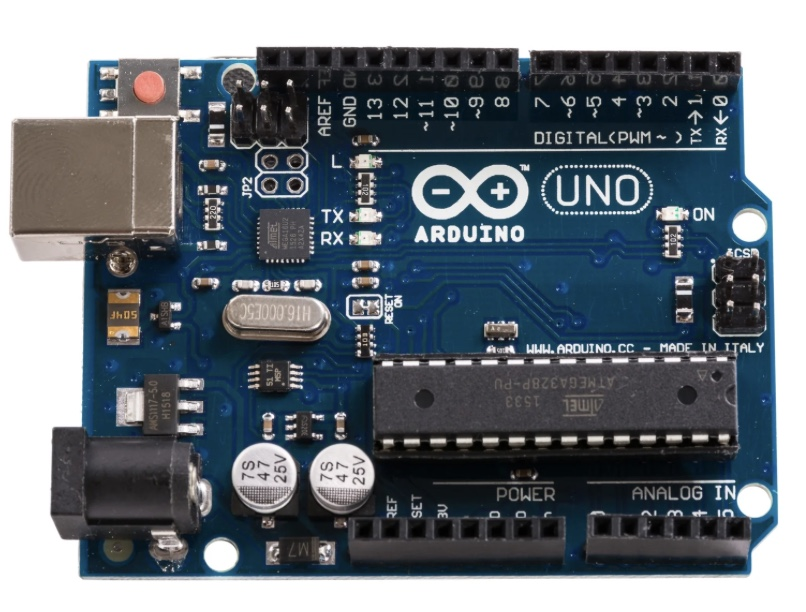
\includegraphics [width=8cm] {img/ArduinoR3}
		\caption{Arduino Uno}
		\label{img:Arduino}
	\end{figure}
\newline
%Pi Intro

\paragraph{Rasperry Pi[\cite*[siehe: ]{ArduinoVsRaspberry2022}]}
Ein Rasperry Pi ist ein Einplatinencontroller, der auf einem ARM-Prozessor basiert.
Er ist dafür konzipiert, eine breite Palette von Anwendungen zu unterstützen, vom Prototypenbau bis zu IoT-Geräten.
Im Gegensatz zum Arduino ist er besonders für komplexe und rechenlastige Projekte geeignet.
\begin{figure}[htbp]
	\centering
	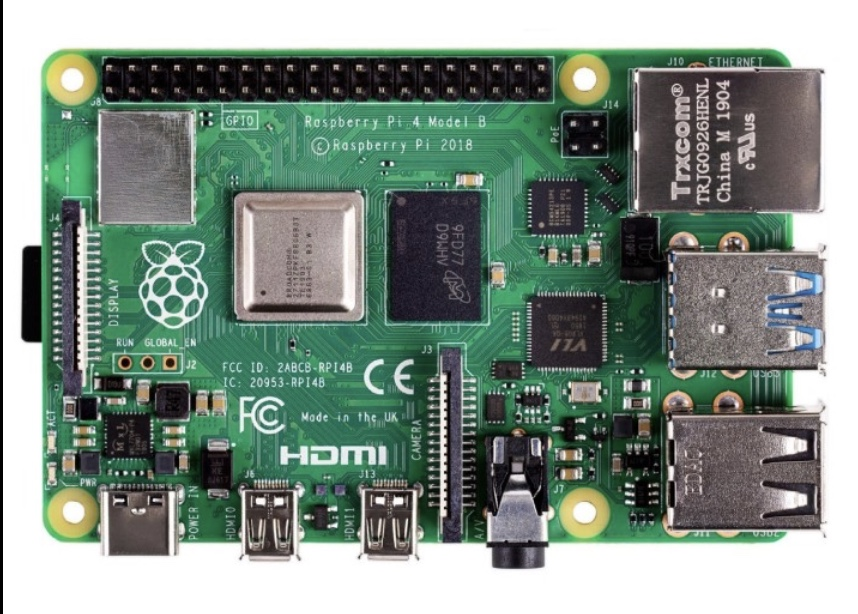
\includegraphics [width=8cm] {img/RasperryPi}
	\caption{Rasperry Pi}
	\label{img:Raspi}
\end{figure}
\newline

%Vergleich
\paragraph{Entscheidungsfindung}
Es wurde sich letztendlich für den Arduino entschieden.
Der Rasperry Pi stand vor allem aufgrund seiner höheren Speicherkapazität und Rechenleistung zur Diskussion, wodurch eine komplexere Ansteuerungslogik möglich wäre.
Allerdings ist er aufgrund seines Betriebssystems nicht für Echtzeit-Anwendungen bzw. geschwindigkeitskritische Anwendungen ausgelegt.
% @Note(Jay): Vllt noch genauer
Im Gegensatz dazu bietet der Arduino eine Echtzeitverarbeitung mit geringer Latenz.
Außerdem verfügt ein Arduino über eine recht simple Hardware-Interaktion - er ist darauf spezialisiert, die Hardware direkt anzusprechen - und ist somit besser für Projekte geeignet, die eine präzise Ansteuerung von Aktuatoren benötigen. % @Note(Val): Simpel != Präzise. Nur weil der Arduino eine simple Hardware-Interaktion hat, heißt es nicht, dass er die Hardware präzise ansteueren könnte
Zudem sollte hier keine besonders komplexe Ansteuerungslogik benötigt werden, weshalb ein Arduino genug Rechenleistung aufweisen sollte.

Für das Projekt wird spezifisch ein Arduino UNO R3 verwendet \cite[siehe][für die genaue Spezifikation]{ard.ArduinoR3Datasheet.24}.
Bei der Auswahl des spezifischen Arduinos wurden der Arduino UNO Mini, Nano und R3 betrachtet.
Im Prinzip wäre jedes der genannten Modelle für die Anwendung möglich, allerdings verfügt der R3 im Gegensatz zu den anderen beiden Modellen über mehr Speicherkapazitäten (256KB Flash Speicher
gegenüber der 32KB vom Arduino UNO Mini und den 30KB, die auf dem Arduino Nano verfügbar sind \cites[vgl.][]{ard.ArduinoR3Datasheet.24}{ard.ArduinoMiniDatasheet.24}{ard.ArduinoNanoDatasheet.24}).
Der Arduino UNO R3 verfügt zwar über mehr Ports, allerdings bringt dies keinen Mehrwert, da die Anzahl der benötigten Ausgänge auch bei einem R3 nicht erreicht werden
(siehe Kapitel \ref{output}).
Der Arduino R3 bietet - wie die anderen beiden Modelle auch - \ac{PWM}-Pins, die im Rahmen des Projekts genutzt werden können.


\subsection{Pulsweitenmodulation}\label{PWM}
\chapterauthor{Jakob Kautz}

Zur Vollständigkeit wird in diesem Abschnitt das Prinzip der \acf{PWM} erläutert.
Zur Vollständigkeit wird in diesem Abschnitt das Prinzip der Pulsweitenmodulation erläutert [Vgl: \cite*[siehe ][]{PWM}].
Oftmals ist bei der Ansteuerung der Aktuatoren nicht die gesamte Versorgungsspannung erwünscht bzw. benötigt.
In diesen Fällen muss die anliegende Spannung varriiert werden, damit die Spannung am Ziel dem gewünschten Wert entspricht.
Angenommen es ist eine Spannung von 2.5V erwünscht, wobei die Vollversorgungsspannung 5V beträgt.
Das Signal kann dafür die Hälfte der Zeit ausgeschaltet werden, womit zwischen 0V und den vollen 5V durchschnittlich insgesamt 2.5V anliegen.
Je höher die Frequenz zwischen An- und Ausschalten des Signals eingestellt wird, desto weniger wird diese \enquote{künstlich} simulierte Halbierung wahrgenommen.

\ac{PWM} bedient sich im Grunde genau dieser Technik.
Dabei wird die Zeitdauer eines digitalen Signals variiert wird, um einen durchschnittlichen Wert zu erzeugen.
Bei den \ac{PWM}-Ausgängen wird die Pulsweite - die Dauer der Einschaltzeit - des Signals angepasst, um die gewünschte Spannung zu erreichen.

\begin{figure}[htbp]
	\centering
	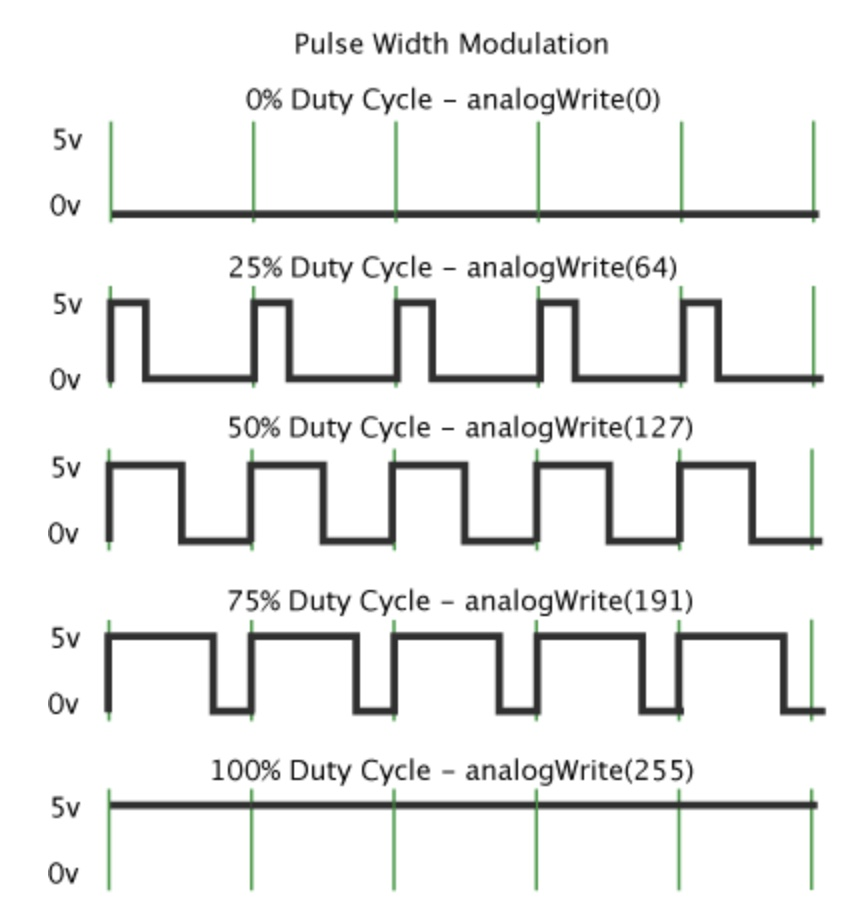
\includegraphics [width=8cm] {img/pulsweite}
	% @Note(Val): Quelle des Bilds fehlt hier noch
	\caption{Pulsweitenmodulation [siehe: \cite*[siehe ][]{PWM}]}
	\label{fig:pulsweite}
\end{figure}

Spezifischer ausgedrück passiert folgendes:
Eine digitale Steuerung wird verwendet, um eine Rechteckwelle - ein Signal das zwischen HIGH und LOW umgeschaltet wird - zu erzeugen.
Dieses HIGH-LOW-Muster kann Spannungen zwischen der vollen Versorgungsspannung und 0V simulieren.
Dabei wird der Anteil der Zeit geändert, für den das Signal auf HIGH geschaltet ist, relativ zur Zeit, in der das Signal auf LOW geschaltet ist.
Um unterschiedliche, analoge Werte zu erhalten, wird die Pulsweite moduliert.
Wenn dieses HIGH-LOW-Muster zum Beispiel schnell genug mit einer LED wiederholt wird, resultiert daraus eine konstante Spannung zwischen 0 und Vcc, die die Helligkeit der LED steuert. % @TODO(Val): Vcc als Abkürzung erst ausschreiben

Auf den Arduino bezogen sieht die Umsetzung eines \ac{PWM} Signals wie folgt aus:
Ein Taktsignal gelangt in die entsprechende Clock.
Die Clock stellt den entsprechenden \ac{PWM}-Modus ein.
Dabei werden zwei wichtige Werte gesetzt:
Der erste bestimmt, wann das Signal von HIGH auf LOW umschaltet, während der zweite bestimmt, wann es zurückkommt.
Das Verhältnis zwischen HIGH und LOW wird als Tastverhältnis bezeichnet und bestimmt die Helligkeit der LED bzw. die Stärke, mit der der Aktuator anschlägt.
Je länger die Ausgabe im HIGH-Zustand bleibt, desto schneller erfolgt entsprechend der Tastenanschlag.

Neben dem Tastverhältnis, welches oft in Prozent ausgedrückt wird, ist auch die Auflösung ein variierbarer Parameter.
Die Auflösung bezieht sich auf die Anzahl der möglichen diskreten Werte, die das Signal annehmen kann.


\subsection{Vermehrung der Ausgänge}\label{output}
\chapterauthor{Jakob Kautz}

Da ein Klavier über 88 Tasten verfügt, müssen 88 Aktuatoren angesteuert werden. Der gewählte Arduino hat keine 88 \ac{PWM}-Ports, daher
müssen die Signale über eine Erweiterung der Ausgänge an die Aktuatoren weitergegeben werden. Dafür gibt es mehrere Möglichkeiten,
wobei in dieser Arbeit 2 im Detail betrachtet werden:

\begin{enumerate}
	\item Schieberegister
	\item Aktuator-Matrix
\end{enumerate}

% @Note(Jay): Wäre es smart zu erwähnen was es noch für Möglichkeiten gibt? Also Arduino Mega muss ich soweiso erwähnen, aber z.B
% @Note(Jay): Shields verbinden oder mehrere Arduinos nutzen weil das haben wir ja kurz überlegt und dann relativ schnell verworfen

\subsubsection{Schieberegister}
Ein Schieberegister[siehe: \cite*[siehe ][]{Schieberegister}] ist ein integrierter Schaltkreis, der zur Speicherung und sequenziellen Verschiebung von
% @TODO(Val): Schieberegister sind bekannt und müssen nicht so detailliert eklärt werden
Ein Schieberegister ist ein integrierter Schaltkreis, der zur Speicherung und sequenziellen Verschiebung von
Datenbits verwendet wird.\newline
Das grundlegende Prinzip eines Schieberegisters ist, dass Datenbits seriell in das Register eingegeben und dann
sequenziell aus dem Register ausgegeben werden können.
Dies geschieht durch die Verwendung von Taktimpulsen, die das Verschieben der Bits steuern.\newline
Schieberegister bestehen aus einer Reihe von Flip-Flops.
Ein Flip-Flop kann als ein einfacher Speicher betrachtet werden, der binäre Informationen speichert und je nach
Eingangssignal den Zustand 1, 0, oder einen \enquote{Flip}-Zustand annimmt.
Diese FlipFlops sind so verbunden, dass sie Daten in einer bestimmten Reihenfolge speichern und weitergeben können.

Um 88 Ausgänge mit Hilfe von Schieberegistern, die von nur 3 \ac{PWM}-Pins des Arduinos agesteuert werden, umzusetzen,
können 11 8-Bit-Schieberegister  - also Schieberegister mit 8 Ausgängen - verwendet werden.

\paragraph{74HC959 Schieberegister}
In dieser Arbeit wird spezifisch ein 74HC959 Schieberegister betrachtet[siehe: \cite*[siehe ][]{DatasheetSchieberegister74HC595}].
Dieses hat folgenden Aufbau:
\begin{figure}[htbp]
\begin{minipage}{0.4\textwidth}
		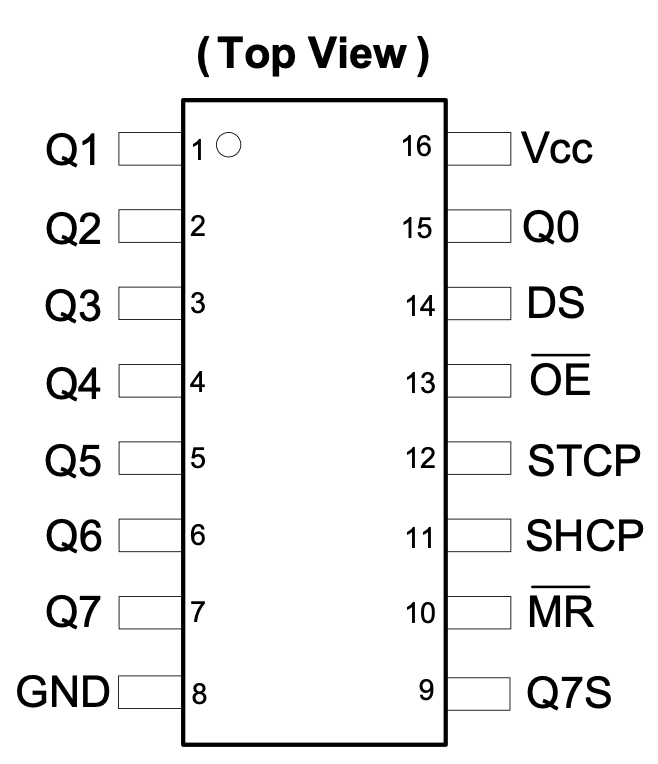
\includegraphics [width=1\textwidth] {img/Schieberegister}
		% @TODO(Val): Bildquelle
		\caption{Schematik Schieberegister}
		\label{img:Shift}
\end{minipage}
\begin{minipage}{0.6\textwidth}
	\begin{enumerate}
		\item Q0-Q7: Ausgänge (parallelgeschaltet)
		\item Vcc: Anschluss Versorgungsspannung (+)
		\item Gnd: Anschluss Versorgugsspannung (-)
		\item DS: Data Signal, serieller Dateneingang
		\item OE: Output Enable, zur Aktivierung der Ausgänge
		\item SHCP: Shift Clock, Clock-Eingang zur Übernahme Data Signals in Schieberegister
		\item STCP: Store Clock, Beim Wechsel von LOW auf HIgh wird der Inhalt des Schieberegisters in das Ausgaberegister kopiert % @Note(Val): Selbe Bezeichnung wie oben verwenden. Entweder LOW/HIGH oder AN/AUS
		\item MR: Master Reset, Leerung des Schieberegisters
		\item Q7S: Überlauf für Kaskadierung
	\end{enumerate}
\end{minipage}
\end{figure}
Ein Nachteil des Schieberegisters besteht darin, dass Latenzen auftreten.
\subsubsection{Aktuator-Matrix} %TODO(Jay): Quelle
Die Aktuator-Matrix ist einer LED-Matrix nachgeahmt.
In einer Matrix, werden zwei Reihen nach folgendem Muster an Ports angeschlossen:
$$
\begin{pmatrix}
	(11) & (12) & (13) & (14) & (15) & (16) & (17) & (18) \\
	(21) & (22) & (23) & (24) & (25) & (26) & (27) & (28) \\
	(31) & (32) & (33) & (34) & (35) & (36) & (37) & (38) \\
	(41) & (42) & (43) & (44) & (45) & (46) & (47) & (48) \\
	(51) & (52) & (53) & (54) & (55) & (56) & (57) & (58) \\
	(61) & (62) & (63) & (64) & (65) & (66) & (67) & (68) \\
	(71) & (72) & (73) & (74) & (75) & (76) & (77) & (78) \\
	(81) & (82) & (83) & (84) & (85) & (86) & (87) & (88)
\end{pmatrix}
$$

Eine LED-Matrix besteht aus einer Anordnung von LEDs in Zeilen und Spalten.
Jede LED kann unabhängig von den anderen ein- oder ausgeschaltet werden.
Die Steuerung der Matrix kann sowohl mit als auch ohne Multiplexing erfolgen.
Prinzipiell wird jede Zeile der Matrix nacheinander aktiviert, während die
entsprechenden LEDs in den Spalten gleichzeitig eingeschaltet werden.
Durch schnelles Wechseln zwischen den Zeilen mithilfe von \ac{PWM}-Signalen erscheint es den Betrachter:nnen, als ob alle LEDs
gleichzeitig leuchten würden, obwohl sie tatsächlich nacheinander aktiviert werden.

\begin{figure}[htbp] %TODO(Jay): Quelle
	\centering
	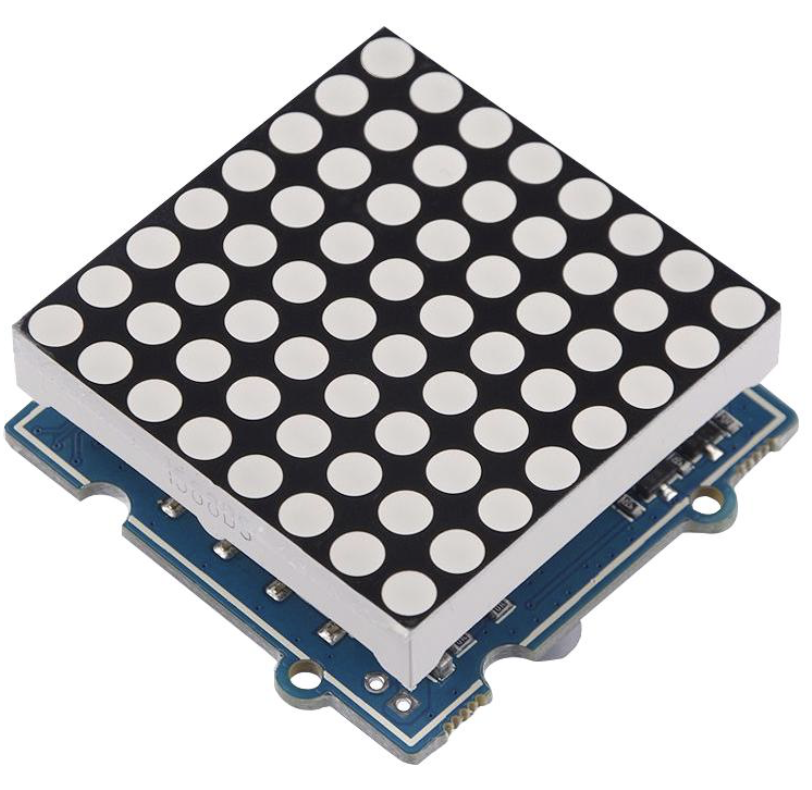
\includegraphics[width=0.45\textwidth]{img/LED-Matrix}
	\caption{Beispielhafte Darstellung einer LED-Matrix}
	\label{img:LED-Matrix}
\end{figure}

%ohne Multiplexer
\paragraph{Matrix ohne Multiplexing}

Bei einer LED-Matrix ohne Multiplexing werden die LEDs direkt über die \ac{GPIO}-Pins des
\ac{MC}s angesteuert. Jede LED ist einzeln mit einem Pin des \ac{MC}s verbunden. Um die LEDs anzusteuern,
muss der \ac{MC} jeden Pin einzeln aktivieren oder deaktivieren, um die entsprechende LED ein- oder auszuschalten.
Hierbei werden viele Pins benötigt, um die gesamte Matrix anzusteuern, was besonders bei größeren Matrizen unpraktisch
sein kann. Für dieses Projekt wird, wie oben aufgeführt, eine 8x8-Matrix benötigt. Es werden also 16 PWM-Fähige Pins
benötigt. Der hier verwendete \ac{MC} verfügt allerdings nur über 6 von diesen Pins.

\begin{figure}[htbp] %TODO(Jay): Quelle
	\centering
	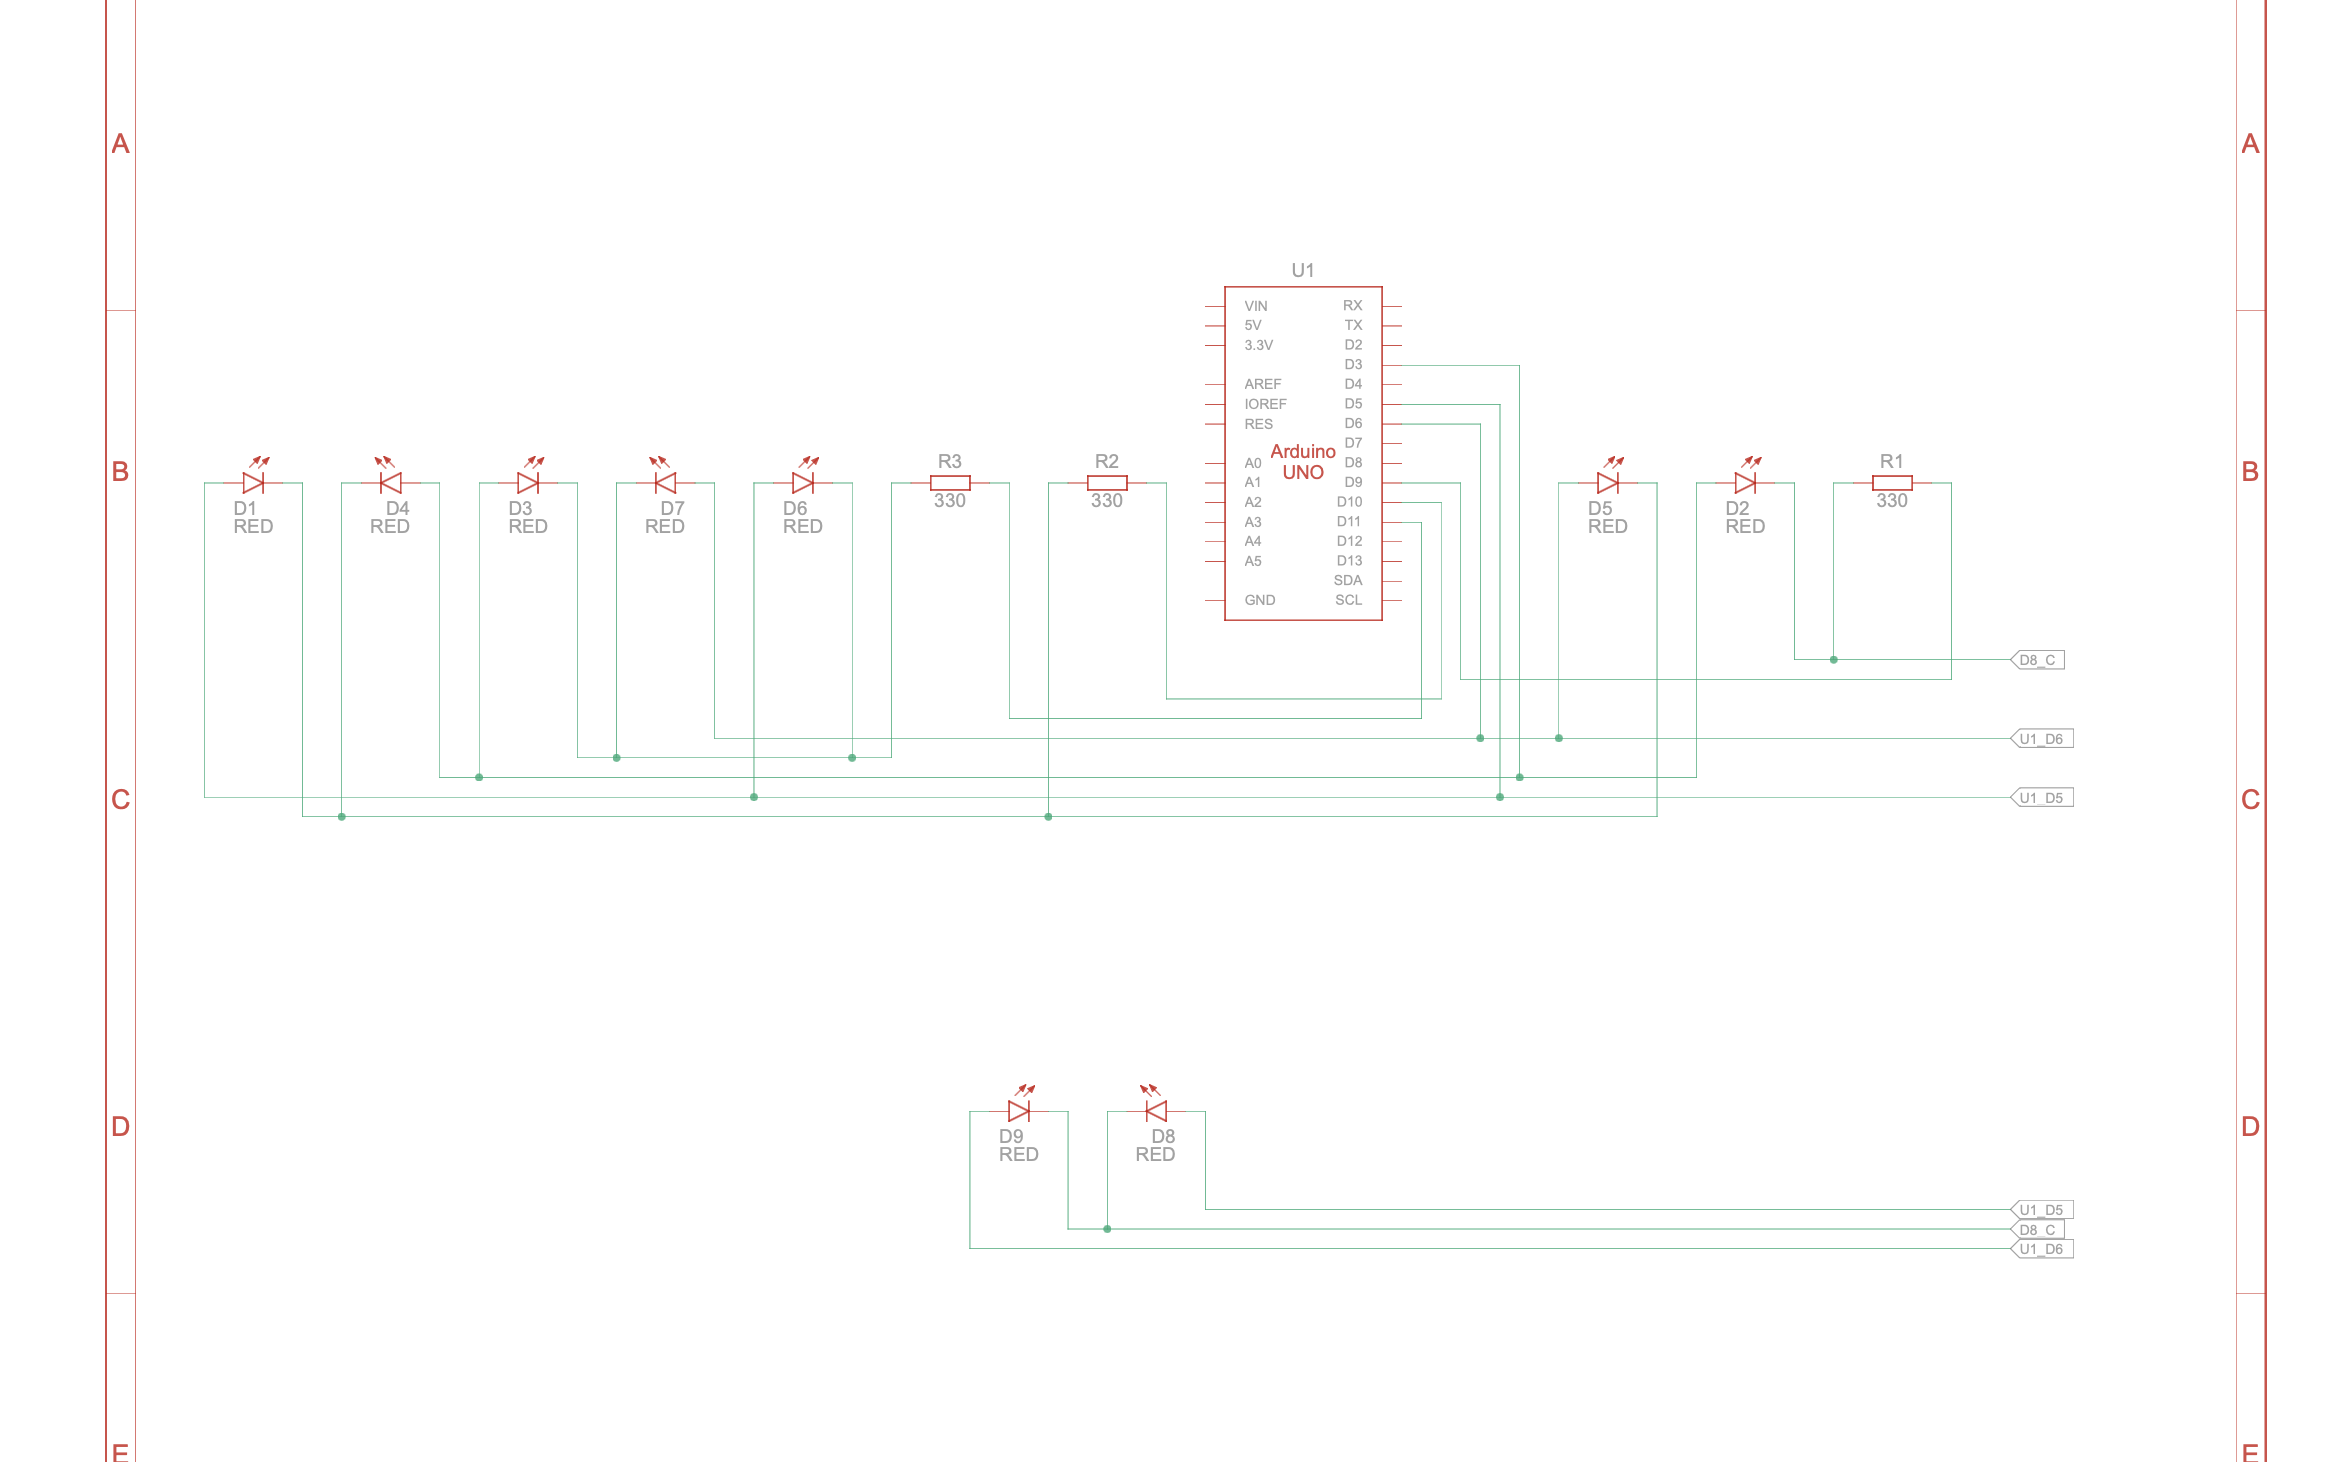
\includegraphics[width=0.6\textwidth]{img/LEDMatrixSchaltung}
	\caption{Matrix ohne Multiplexing Schematisch}
	\label{fig:Matrix}
\end{figure}
% @Note(Jay): Welches der Bilder?
%Um die Komplexität darzustellen, eine Aktuator-Matrix ohne Multiplexer würde für neun Aktuatoren wie folgt aussehen:
% \begin{figure}[htbp]
% 	\centering
% 	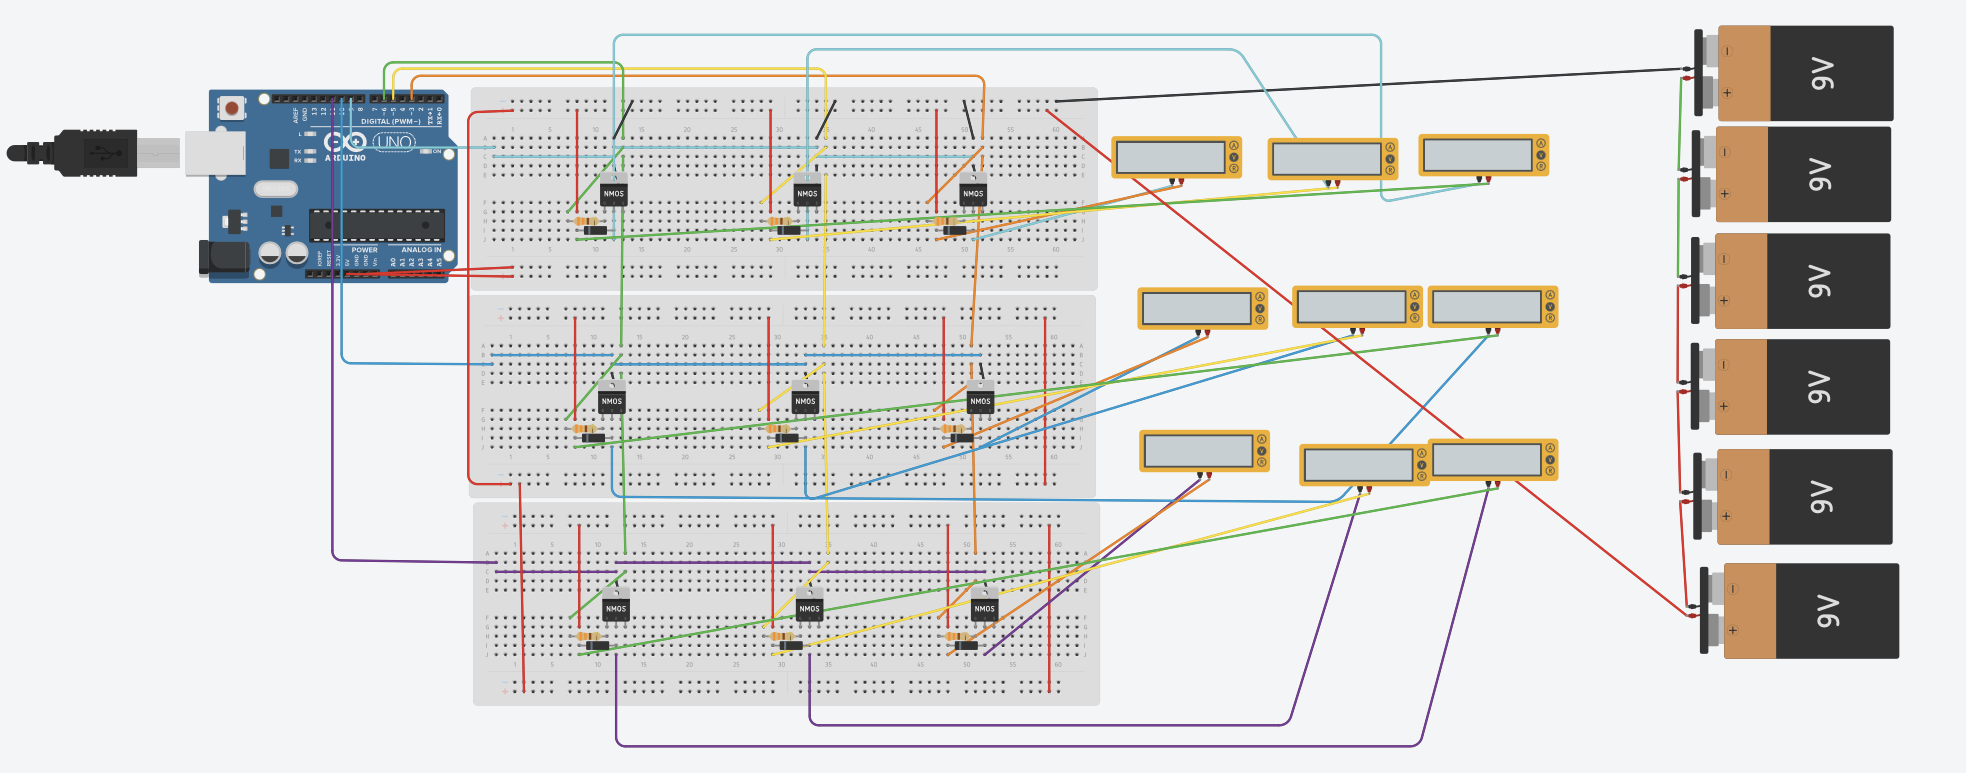
\includegraphics[width=0.9\textwidth]{img/AktMatrix}
% 	\caption{Aktuator-Matrix ohne Multiplexer}
% 	\label{fig:AktMatrix}
% \end{figure}
% @TODO(Val): Das erste Bild ist zu klein, um erkenntlich zu sein und das zweite Bild ist überhaupt nicht verständlich (wo ist da zum Beispiel die Matrix)
% @TODO(Val): Bildquelle

%mit Multiplexer
%Was ist ein Multiplexer, warum hilft er bei Martix wie sieht allg Schaltung aus?
\paragraph{Matrix mit Multiplexing}
Ein Multiplexer (bzw. ein Demultiplexer) ermöglicht das Kombinieren mehrerer Signale zu einem bzw. dem Trennen eines einzelnen Signals zu mehreren, unterschiedlichen Signalen.
Bei einer LED-Matrix erfolgt das Prinzip durch die Verwendung von Schieberegistern und Transistoren. % @TODO(Val): Sicher, dass das richtig ist?
Somit kann damit die Notwendigkeit zum Verbinden jedes individuellen Pins mit einem GPIO-Pin des \ac{MC}s elimniert werden.
Entsprechend werden weniger Pins benötigt, um die Matrix anzusteuern.
Die Nutzung von Multiplexern bringt somit eine effizientere Ressourcennutzung mit sich, kommt allerdings auch mit einer komplexeren Schaltung und Latenzen durch die Schieberegister einher. % @Note(Val): Sind die Latenzen nur "möglich"? Müsste es nicht entweder klar Latenzen erhöhen oder nicht?
Wobei die Latenzen der Schieberegister in diesem Projekt vernachlässigt werden können.
\begin{figure}[htbp] %TODO(Jay): Quelle
	\centering
	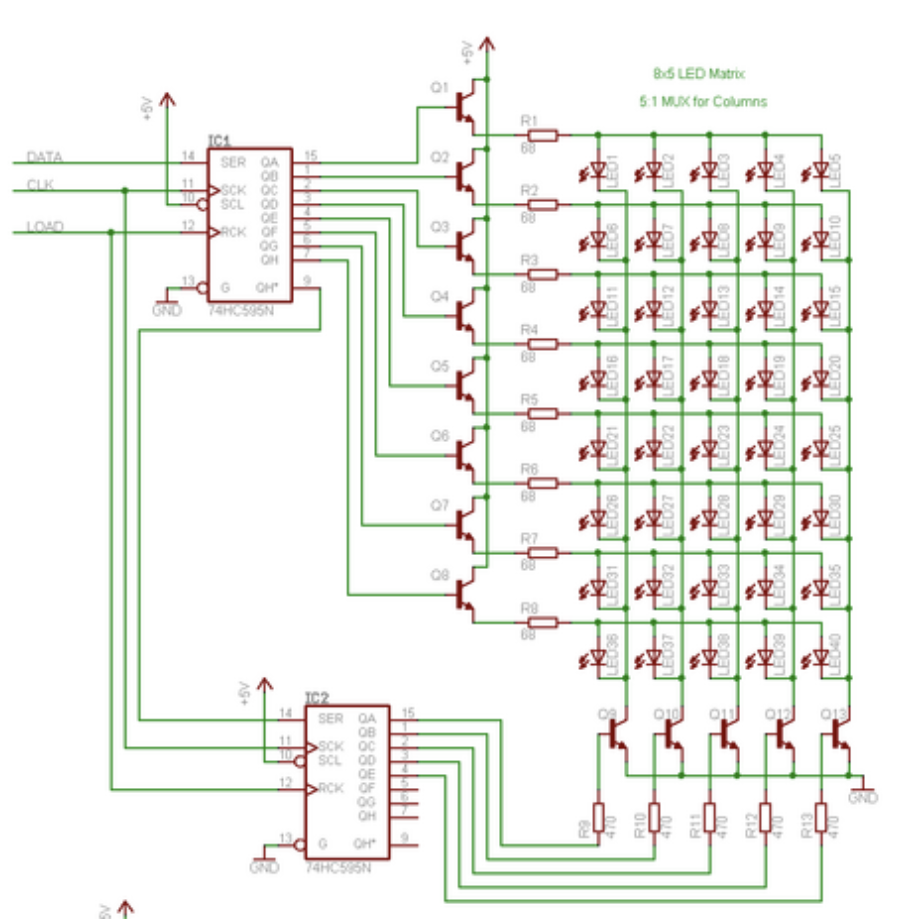
\includegraphics[width=0.75\textwidth]{img/matrixMuxSchaltung}
	\caption{Aktuator-Matrix mit Multiplexing}
	% @TODO(Val): Bildquelle
	% @TODO(Val): Im Bild steht LED-Matrix, deswegen ist es komisch in der Bildüberschrift dann "Aktuator-Matrix" zu schreiben
	\label{fig:AktMatrixMux}
\end{figure}

\subsubsection{Entscheidungsfindung}
Letztendlich fiel die Entscheidung auf die Verwendung von Schieberegistern. Dies liegt an mehreren Gründen:
\begin{enumerate}
	\item \textbf{Funktionalität:} Bei der Verwendung einer Aktuatoren-Matrix über \ac{PWM}
	kann es zu Interferenzen kommen, die die Präzision der Steuerung beeinträchtigen. Da die \ac{PWM}-Signale zeilenweise
	vom Multiplexer kombiniert werden, kann es vorkommen, dass die \ac{PWM}-Signale nicht mit der benötigten Stärke für jeden Aktuator geliefert
	werden. Das liegt daran, dass verschiedene Aktuatoren in derselben Zeile unterschiedliche \ac{PWM}-Signale benötigen können,
	was zu ungenauer Steuerung führt. Dies kann zu Kompromissen bei der Präzision und Leistung der Aktuatoren führen.
	\item \textbf{Komplexität:} Die Implementierung einer Aktuator-Matrix über eine
	LED-Matrix hinaus wäre technisch anspruchsvoller und erfordert eine komplexere Schaltung. Im Gegensatz dazu ist die
	Verwendung von Schieberegistern eine einfachere Methode zur Ansteuerung der Aktuatoren.
	\item \textbf{Anzahl der Pins:} Wie bereits erklärt, benötigt die Matrix ohne Multiplexing eine Vielzahl an Pins, welche der \ac{MC}
	nicht liefert. Da die Matrix verwendet werden sollte um eben dieses Problem zu lösen, liefert die Matrix keine gute Lösung.
	Durch die Kombination von Schieberegistern und Matrixaufbau wäre dieses Problem gelöst.
	Es würden insgesamt 2 Schieberegister benötigt werden, also 6 Pins die diese ansteuern, womit die Anzahl der verfügbaren Pins ausreichen würde.
	Die Entscheidung von dieser Variante abzusehen, ist in den anderen hier aufgeführten Punkten begründet.
	\item \textbf{Ressourcen:} Desweiteren basiert die Entscheidung auf unzureichenden Ressourcen für die Matrix. Im Internet gab es
	keine ausreichenden Anleitungen/Ressourcen, die die Implementierung einer LED-Matrix mit Aktuatoren ausreichend
	unterstützen würden. Zusätzlich dazu lieferten die Simulationen via Tinkercad\footnote{Tinkercad: https://www.tinkercad.com} keine befriedigenden Ergebnisse
	für die Aktuator-Matrix.
	Im Gegensatz dazu sind Schieberegister gut dokumentiert und es gibt ausreichende Ressourcen, um ihre
	Verwendung für die Ansteuerung von Aktuatoren zu verstehen und umzusetzen.
	% @Note(Jay): Ist zu sagen das wir nichts nutzen wollten wo wir keine konkrete Aussage zu finden wenn wir wissen dass es anders funktioniert okay?
	% @Note(Val): Ist ok und ein valider Punkt, aber klingt ein bisschen als wären wir einfach inkompetent lol
\end{enumerate}

\subsection{Transistor} 
\chapterauthor{Jakob Kautz}
Ein Transistor [\cite*[siehe ]{BipolarerTransistor}] ist ein elektronisches Bauteil, das in der Lage ist, den Stromfluss zwischen zwei seiner Anschlüsse
(den sogenannten Source und Drain) mithilfe eines dritten Anschlusses (der Gate) zu steuern.

Verwendung von Transistoren in Aktuatoren-Schaltungen:
Transistoren werden in Aktuatoren-Schaltungen verwendet, um die Aktuatoren
zu steuern. Sie dienen als Schalter, der den Stromfluss zu den Aktuatoren regelt.
Dabei ist es wichtig, auf die Durchlassspannung und Mindestspannung des MOSFETs zu achten. Die Durchlassspannung ist die
minimale Spannung, die an das Gate angelegt werden muss, um den MOSFET in den leitenden Zustand zu versetzen. Die
Mindestspannung ist die minimale Spannung, die zwischen Source und Gate anliegen muss, um den MOSFET zuverlässig zu
sperren.
Es ist entscheidend, sicherzustellen, dass die Spannungen in der Schaltung diese Anforderungen erfüllen, um
eine ordnungsgemäße Funktion des MOSFETs sicherzustellen und Schäden zu vermeiden.

\subsection{Aktuator}\label{subsec:aktuator}
\chapterauthor{Jakob Kautz}
Die Aktuatoren werden für die Steuerung der Tasten benötigt.
Bei den möglichen Aktuatoren für die Ansteuerung der Klaviertasten wurden drei Möglichkeiten betrachtet: % @Note(Val): Falls es einen Grund gibt, nur diese 3 zu betrachten, gerne nennen, ansonsten sollte das auch so fine sein, glaube ich
\begin{enumerate}
	\item Elektromotor: Schrittmotor
	\item Elektromotor: linearer Servomotor
	\item Hubmagnet
\end{enumerate}
An sich laufen alle 3 Aktuatoren auf das gleiche Prinzip - elektromagnetische Induktion - hinaus. Der Hauptunterschied
der in dieser Arbeit betrachtet wird, ist einmal der Unterschied zwischen einer rotierenden und linearen Bewegung der Aktuatoren,
und im späteren noch wie die Aktuatoren bezüglich Präzision, Kraft, etc. abschneiden.
\paragraph{Elektromotor} \cite*[siehe ][]{Aufbau.Elektromotoren}
Zu Beginn wird ersteinmal das eigentliche Prinzip hinter Elektromotoren betrachtet, da dies hinter allen gewählten Aktuatoren
ähnlich ist.

Grundlegend handelt es sich bei einem Elektromotor um ein Bauteil, welches elektrische Leistung in mechanische umwandelt.
Er besteht aus dem von Statoren erzeugten Magnetfeld und einem sich drehenden Magneten (Rotor) im Inneren.
Betrachten wir also den Elektromagneten, welcher als Hauptkomponente zur mechanischen Leistung beiträgt:

\begin{figure}[htbp]
	\centering
	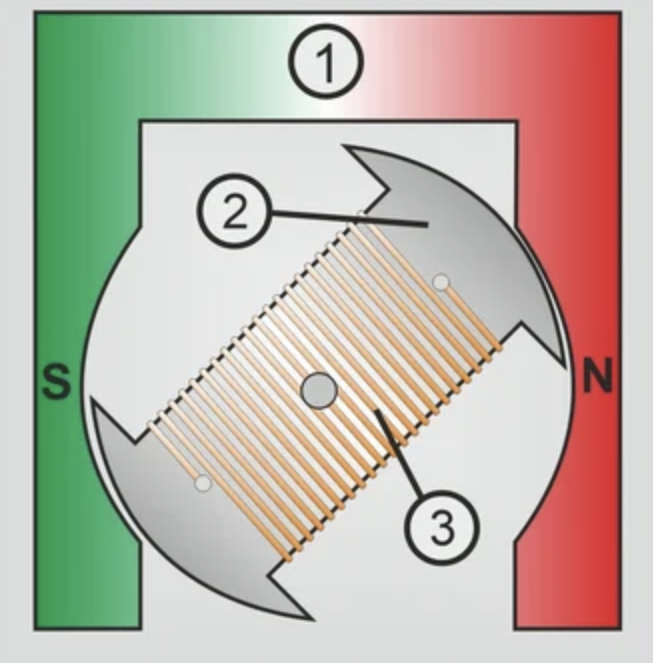
\includegraphics[width=5cm]{img/AufbauElektromagnet}
	\caption{Aufbau eines Rotors\cite*[siehe ][]{Aufbau.Elektromotoren}}
	\label{fig:Elektromagnet}
\end{figure}
Dabei markieren die Nummern die verschiedenen Komponenten.
\begin{enumerate}
	\item Dauermagnet % @Question(Jay): Ab wann ist etwas direkt zitiert? Weil in der Quelle steht es so: Um einen Elektromotor bauen zu können, wird zunächst ein Dauermagnet (1) in einer bestimmten Bauform benötigt. Zwischen den Polen des Dauermagneten ist ein drehbares Eisenteil (2) gelagert, um das eine Spule aus isoliertem Kupferdraht (3) gewickelt ist.
	\item Drehbares Eisenteil
	\item Spule
\end{enumerate}
Wird ein Gleichstrom angelegt, fließt dieser durch die Spule, welche so ein Magnetfeld erzeugt.
\begin{figure}[htbp]
	\centering
	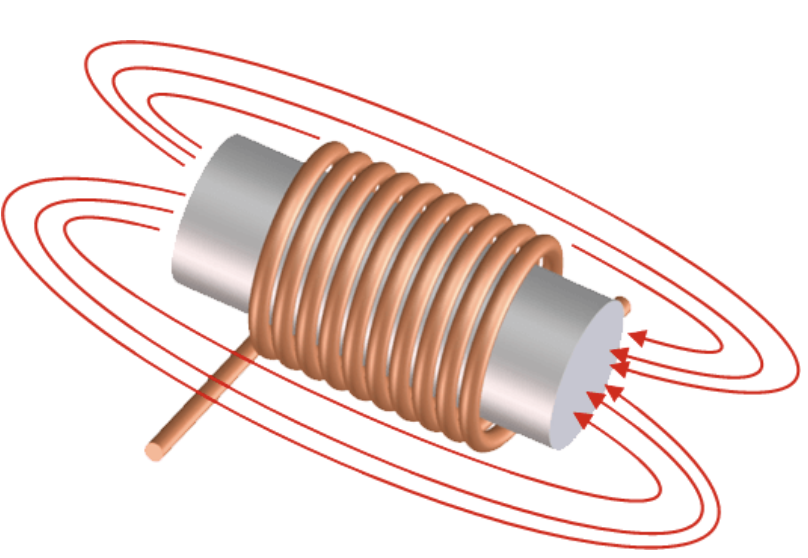
\includegraphics[width=5cm]{img/Magnetfeld}
	\caption{Spule mit Magnetfeld\cite*[siehe ][]{Elektromagnete}}
	\label{fig:Magnetfeld}
\end{figure}
Der Eisenkern wird nun zum Elektromagneten. Die Polung des Magneten hängt davon ab, in welche Richtung der Strom fließt.
Um die Drehbewegung zu ermöglichen, ist die Positionierung des Magneten so, dass der Süd- am Nordpol und der Nord- am Süd-Pol
sind. Die gewünschte Rotierbewegung erfolgt durch das umpolen der magnetischen Ausrichtung.
Dafür ist ein sogenannter Kollektor zuständig, welcher die Stromrichtung in der Spule umschaltet.


\paragraph{Schrittmotor\cite*[siehe ][]{Aufbau.Elektromotoren}}
Ein Schrittmotor übt eine Rotierende Bewegung aus.
\begin{figure}[htbp]
	\centering
	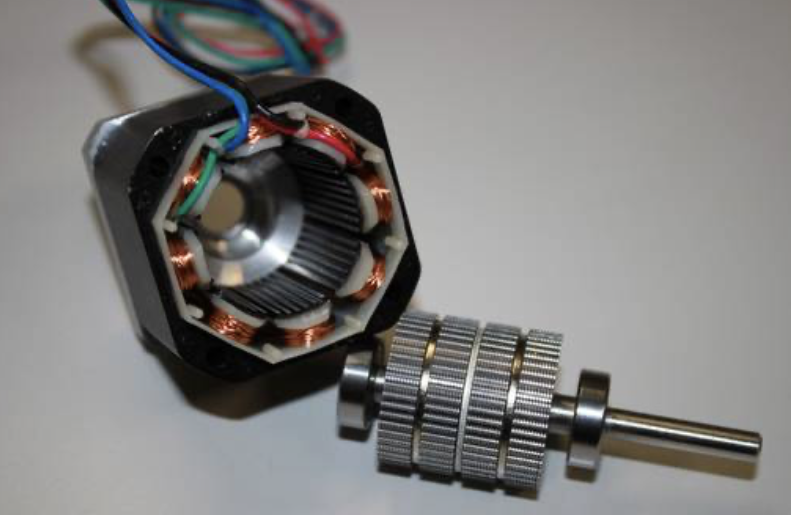
\includegraphics[width=5cm]{img/Schrittmotor}
	\caption{Schrittmotor\cite*[siehe ][]{Aufbau.Elektromotoren}}
	\label{fig:Linearmotor}
\end{figure}
Ein Schrittmotor, ist im Wesentlichen ein Brushless-Elektromotor, der intern so konstruiert ist,
dass er Drehbewegungen in präzise definierten Schritten ausführt, typischerweise mit einem Winkel von 1,8 Grad oder weniger.
Dabei sind Brushless-Elektromotoren Drehstrommotoren. Als Innenläufer sind die Wicklungen des stators außerhalb im festen Gehäuse,
während der Rotor sich im inneren dreht.
Die Energieversorgung erfolgt über Gleichspannung, die in einer festgelegten Reihenfolge auf die Spulen des Motors
geschaltet wird, um die Bewegung zu steuern.
Schrittmotoren finden eine hohe Anwendung in der Steuerungstechnik, was einer der Gründe ist, warum dieser Motor in dem
Projekt betrachtet wird. Durch ihre bürstenlose Bauweise verursachen sie keine Störungen durch Bürstenfeuer, was bei einem
Holzklavier durchaus sinnvoll erschien.


\paragraph{Linearer Servomotor\footnote{\cite*[siehe ][]{Linearer.Servo}}}
Im Gegensatz zum Schrittmotor, wird die elektrische Leisung hier in eine lineare Bewegung umgewandelt. Er basiert auf der
Verwendung permanentmagnetischer Felder. Im Wesentlichen
verhält sich ein linearer Servomotor ähnlich wie ein rotierender Servomotor, jedoch ist er in seiner Form gestreckt und
linear ausgelegt.
\begin{figure}[htbp]
	\centering
	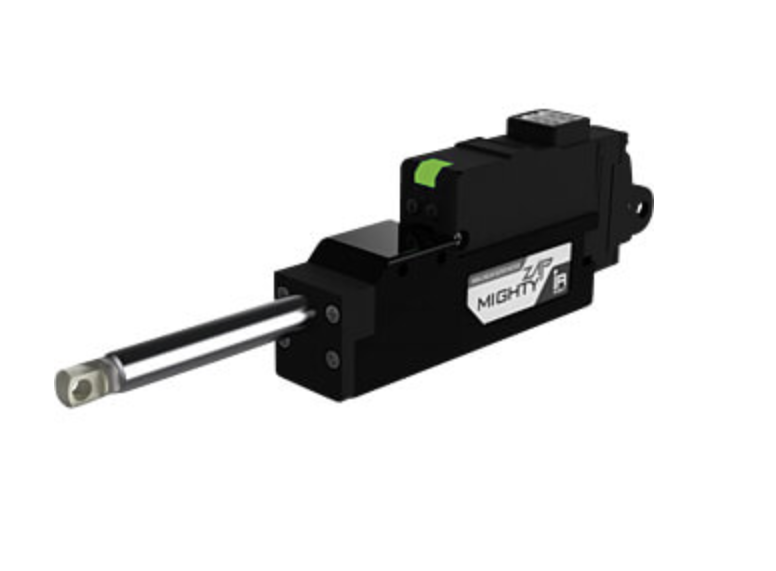
\includegraphics[width=5cm]{img/LinServo}
	\caption{Linearer Servomotor\footnote{\cite*[siehe ][]{ReicheltLinearerServomotor}}}
	\label{fig:Servomotor}
\end{figure}
Im wesentlichen besteht der Motor aus 5 verschiedenen Komponenten:
\begin{enumerate}
	\item Spule/Kolben: Für die eigentliche Umsetzung von Energie in mechanische Leistung zuständig
	\item magnetische Welle (durch Rotor): Schwingung aus elektrischen und magnetischen Feldern, die sich räumlich ausbreitet
	\item Rückführsystem: Meldet relevante Parameter des Zustands des Motors zurück
	\item Linearlager und- führung: Ermöglichen Bewegung entlang einer geraden Achse
	\item Servoverstärker/Steuerungseinheit: Schnittstelle Steuerung und Motor
\end{enumerate}
Diese Elemente ermöglichen eine direkte lineare Bewegung,
wobei der Servoregler den Motor mit Strom versorgt und die Rückmeldungen mit den Sollparametern vergleicht,
um die Leistung zu optimieren.

\begin{figure}[htbp]
	\centering
	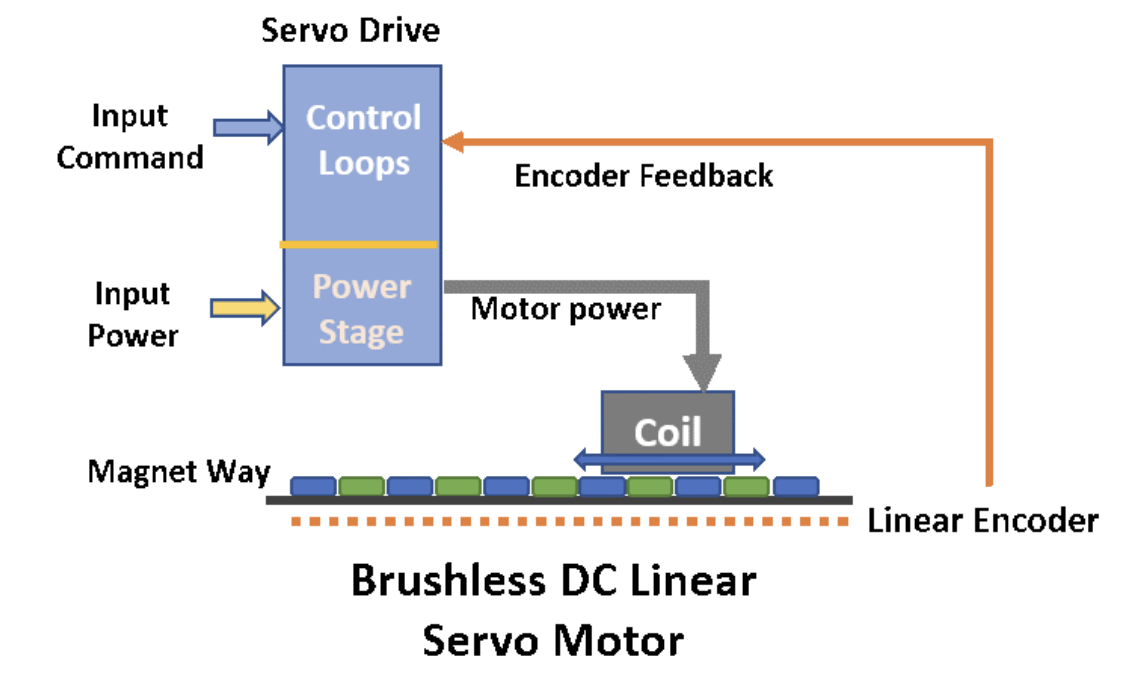
\includegraphics[width=5cm]{img/BrushlessDCLin}
	\caption{Aufbau eines Linearen Servo-motors\footnote{\cite*[siehe ][]{Linearer.Servo}}}
	\label{fig:ServomotorAufbau}
\end{figure}
Für eine präzise Bewegungssteuerung werden integrierte Servoregelkreise eingesetzt, die Strom-, Geschwindigkeits- und
Positionsregelung umfassen. Der Stromkreis reguliert den Strom, um die Kraft für Beschleunigung oder Schub zu liefern,
während die Geschwindigkeitsschleife die Geschwindigkeit proportional zur Spannung steuert. Die Positionsregelschleife
übernimmt den Sollwert und passt die Bewegung entsprechend an.

\paragraph{Hubmagnet\footnote{\cite*[siehe ][Chapter 1-2]{SolenoidDesign}}}
Hubmagnete fallen ebenfalls unter die Elektromotoren.
\begin{figure}[htbp]
	\centering
	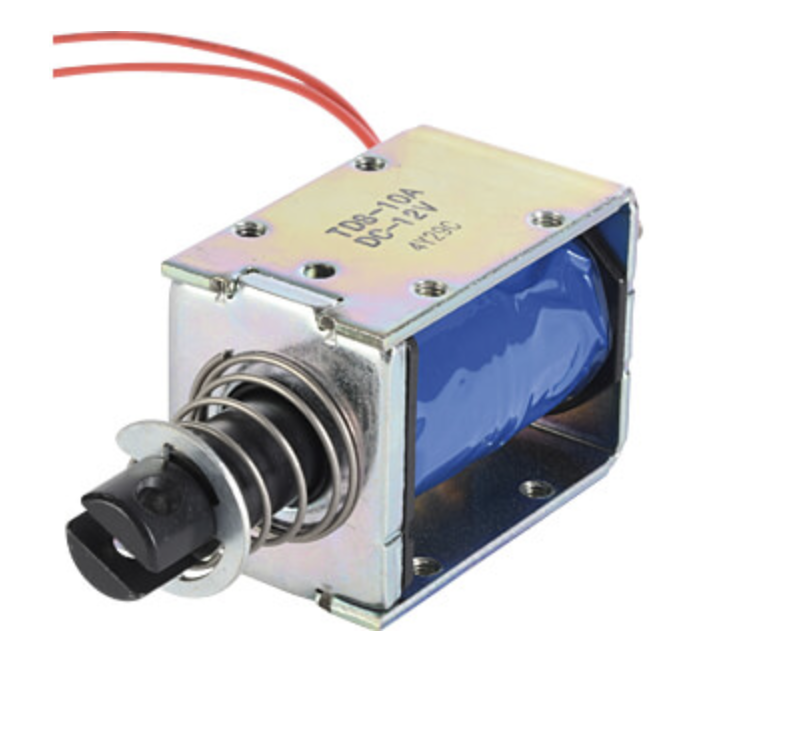
\includegraphics[width=5cm]{img/Hubmagnet}
	\caption{Hubmagnet\footnote{\cite*[siehe ][]{ReicheltHubmagnetMonostabil}}}
	\label{fig:Hubmagnet}
\end{figure}

Hubmagnete verwenden eine lange
Drahtschleife, die um einen metallischen Kern (Plunger) gewickelt ist, und erzeugen ein Magnetfeld, um die lineare Bewegung
des Plungers zu erzeugen, wenn ein elektrischer Strom durch die Drahtspule fließt. Lineare Solenoids können einseitig oder
bidirektional (Drücken und Ziehen) sein und haben oft eine Rückholfeder, um den Plunger in die Ausgangsposition zurückzubringen.
\begin{figure}[htbp]
	\centering
	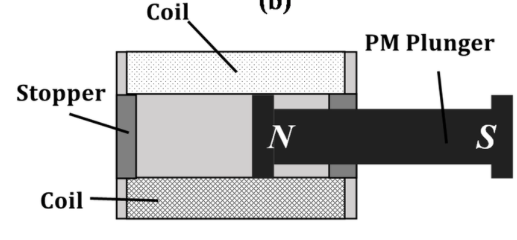
\includegraphics[width=5cm]{img/AufbauMagnet}
	\caption{Hubmagnet Aufbau\footnote{\cite*[siehe ][]{SolenoidDesign}}}
	\label{fig:HubmagnetAufbau}
\end{figure}

\paragraph{Entscheidungsfindung}
Prinzipiell kann jeder der genannten Aktuatoren für das Projekt verwendet werden. Die Entscheidung fiel aufgrund
mehrerer Vortzeile allerdings auf den Hubmagneten:
\begin{enumerate}
	\item Schritt-Motor: Im laufe der Arbeit wurde sich gegen eine rotierende Bewegung des Aktuators entschieden. Diese
	hätte in der Konzeption mehrere Umleitungen der Seile gebraucht, damit die Tasten gerade nach unten gezogen werden können.
	Außerdem bringt es mit den in Kapitel \ref{Zielstellung} definierten Anforderungen keinen Mehrwert,
	die Bewegung des Aktuators in \enquote{Schritte} aufzuteilen. Der Hauptgrund der Betrachtung dieses Aktuators lag darin,
	dass das Projekt hier dazu erweitert werden kann, nicht nur MIDI-Dateien zu spielen, sondern auch andersherum am Klavier
	gespielte Stücke zu speichern und automatisch wiederzugeben, da die Position der Aktuatoren einfach gespeichert und
	ausgelesen werden kann. % @Question(Jay): Ist der Satz sinnvoll? Ich stolper beim lesen drüber aber mir fällt grad keine Formulierung ein
	\item Linearer Servo-Motor: Prinzipiell gibt es drei Gründe warum die Entscheidung nicht auf den linearen Servo-motor fiel.
	Der Hauptgrund lag im Preis, der sehr viel Höher ist als für die Hubmagnete, da die Steuerungssysteme in den Motoren komplexer sind.
	Aus dem gleichen Grund, haben Hubmagnete in der Regel eine höhere Reaktinsgeschwindigkeit, was bei Musikstücken eine
	große Rolle spielt.
	Außerdem ist die Montage von Hubmagneten - insbesondere wenn es an Platz mangelt - einfacher, da diese tendenziell
	kleiner sind. % @Question(Jay): Ist es sinnvoll noch Vorteile zu nennen? Also sowas wie bessere Dynamik des Motors wodurch die Tasten "schöner" gespielt werden könnten und höhere Präzision was sinnvoll gewesen wäre wenn wir das von hinten hochdrücken gemacht hätten?
	\item Hubmagnete: Hubmagnete bieten Vorteile wie schnelle Reaktion, einfache Steuerung und geringe
	Herstellungskosten im Vergleich zu anderen Aktuatoren. Der Hubmagnet wurde aufgrund seines einfachen Aufbaus,
	kostengründen, und seiner Geschwindigkeit gewählt. Die verwendeten Hubmagnete können eine Kraft von 25N ausüben,
	was dazu genügt, eine Taste  zu spielen und gleichzeitig Platz für dynamische Anpassungen von Lautstärke und
	Tastanschlag lassen.
\end{enumerate}

\subsection{Schaltplan} \label{subsec:schaltplan}
\chapterauthor{Olivier Stenzel, Jakob Kautz}

Der Schaltplan besteht im Großteil aus den bereits aufgeführten Komponenten:
\begin{enumerate}
	\item Arduino
	\item Schieberegister
	\item MOSFET
	\item Hubmagnet
\end{enumerate}
In diesem Kapitel wird erläutert, wie diese Komponenten miteinander verbunden werden um eine Funktionsfähige
Schaltung zu erstellen. Die gesamte Schaltung mit allen 88 Hubmagneten wird wie folgt aussehen:
\begin{figure}[htbp]
	\centering
	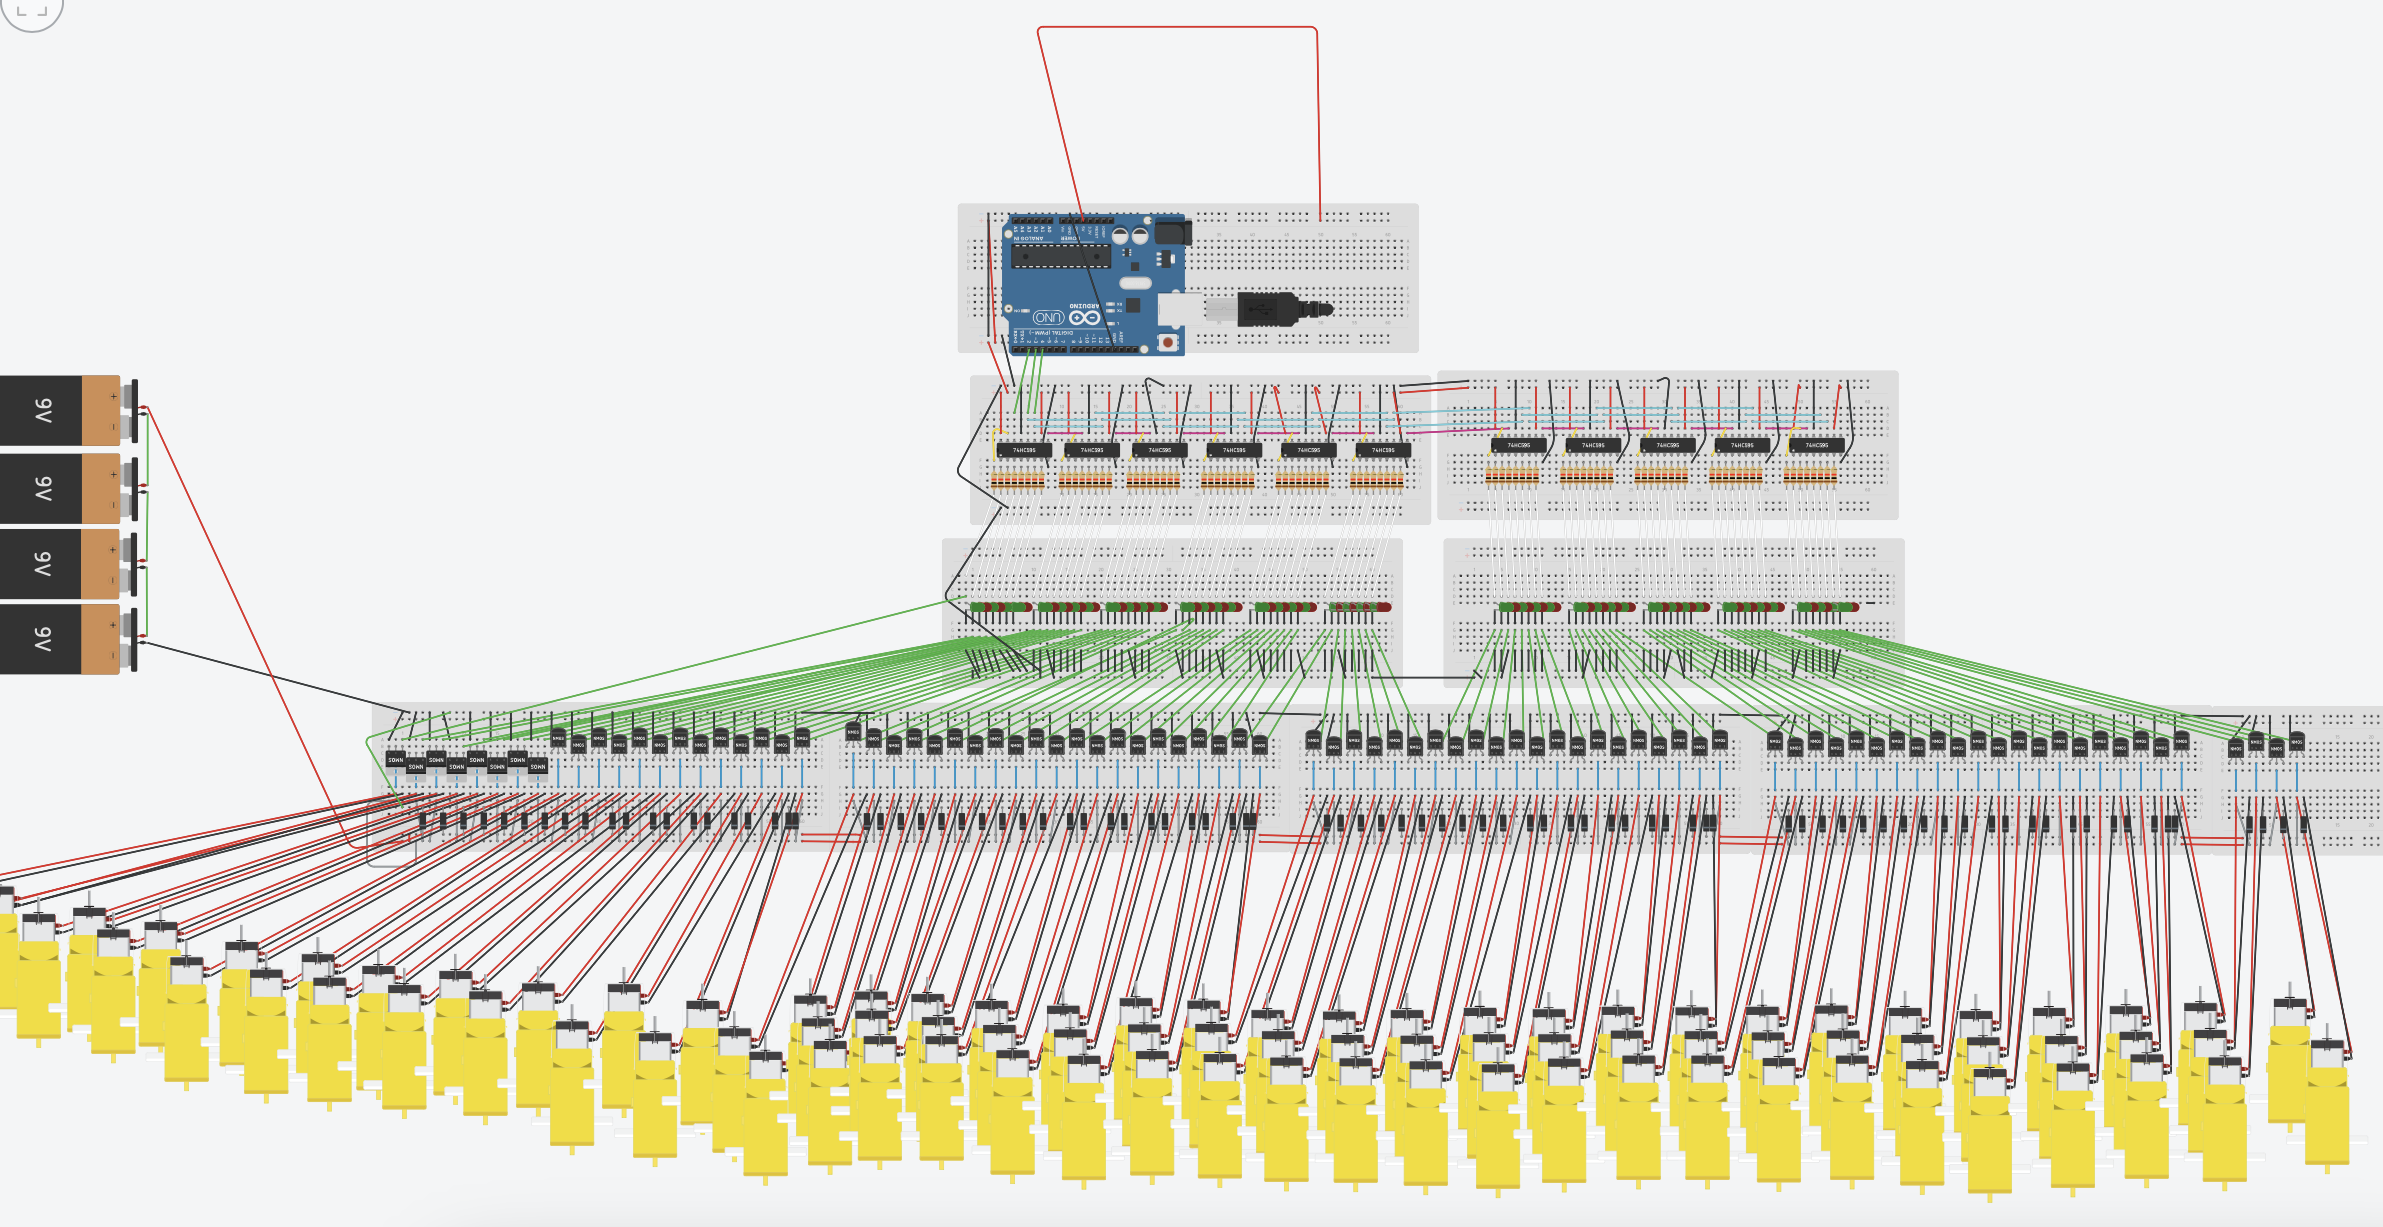
\includegraphics [width=0.85\textwidth] {img/SchaltungGesamt}
	\caption{Überblick Schaltplan}
	\label{img:Schaltplan}
\end{figure}
\subsubsection{Arduino}

Im Zentrum der Schaltung steht der \ac{MC} (hier: Arduino Uno R3).
Dieser erhält Daten und Strom über den integrierten USB-Anschluss, welcher mit dem Computer verbunden wird.
Da der Arduino limitierte \nameref{PWM}-fähige Ausgänge bereitstellt, werde Schieberegister (74HC595) verwendet.
Mit jedem \enquote{in Reihe} geschaltetem Schieberegister kann die Anzahl \ac{PWM}-fähiger Ausgänge um 8 erweitert werden.

\subsubsection{Schieberegister}

Der Arduino wird an fünf Stellen mit dem ersten Schieberegister verbunden:

Arduinoport D2 <-> Serial (SER) Input

Über diese Verbindung werden serielle Daten werden hier bitweise in das Register geschoben.

Arduinoport D3 <-> SHCP (Shift Register Clock Input)

Dieser Pin wird verwendet, um den Takt für das Verschieben der Daten innerhalb des Schieberegisters anzulegen.
Bei jedem Taktimpuls auf diesem Pin wird das Bit am seriellen Dateneingang in das Register verschoben.
Das bedeutet, dass bei jeder steigenden Flanke des Taktsignals das Datenbit, das am Eingang anliegt, in das Schieberegister übernommen und alle vorhandenen Daten um eine Position verschoben werden.

Arduinoport D4 <-> STCP (Storage Register Clock Input)

Nachdem die Daten in das Schieberegister eingelesen wurden, wird dieser Pin verwendet, um die im Schieberegister vorhandenen Daten in das Ausgangsregister zu übertragen.
Ein Taktimpuls auf diesem Pin bewirkt, dass die Daten vom Schieberegister ins Ausgangsregister übernommen werden, sodass alle Ausgänge gleichzeitig aktualisiert werden.
Das ist besonders relevant, da sonst unter Umständen alle Ausgänge von einer Änderung im letzten Schieberegister betroffen wären.

Arduino GND <-> Ground, Output Enable (OE)

Der OE-Pin wird genutzt, um die Ausgänge des Schieberegisters global zu aktivieren oder zu deaktivieren, ohne die Daten selbst zu beeinflussen.
Da das Schieberegister zu keiner Zeit deaktiviert sein soll, wird dieser Pin dauerhaft mit dem GND-Pin verbunden.

Arduino VCC 5V <-> VCC, $\overline{SRCLR}$ (Reset)

Um das Schiebregister mit den benötigten 5V zu betreiben, wird der entsprechende Pin mit dem 5V Output des Arduino verbunden.
Zusätzlich wird der $\overline{ }$ SRCLR Port des Schieberegisters, welcher ein Reset ermöglicht dauerhaft mit 5V verbunden.

Jedes weiteres Schieberegister greift die oben genannten Signale ab.
Der einzige Unterschied befindet sich am Serial (SER) Input Port.
Das Schieberegister an Position i+1 wird mit dem seriellen Output des Schieberegisters an Position i verbunden. ($\forall i = 0,...,10$)

\begin{figure}[htbp]
	\centering
	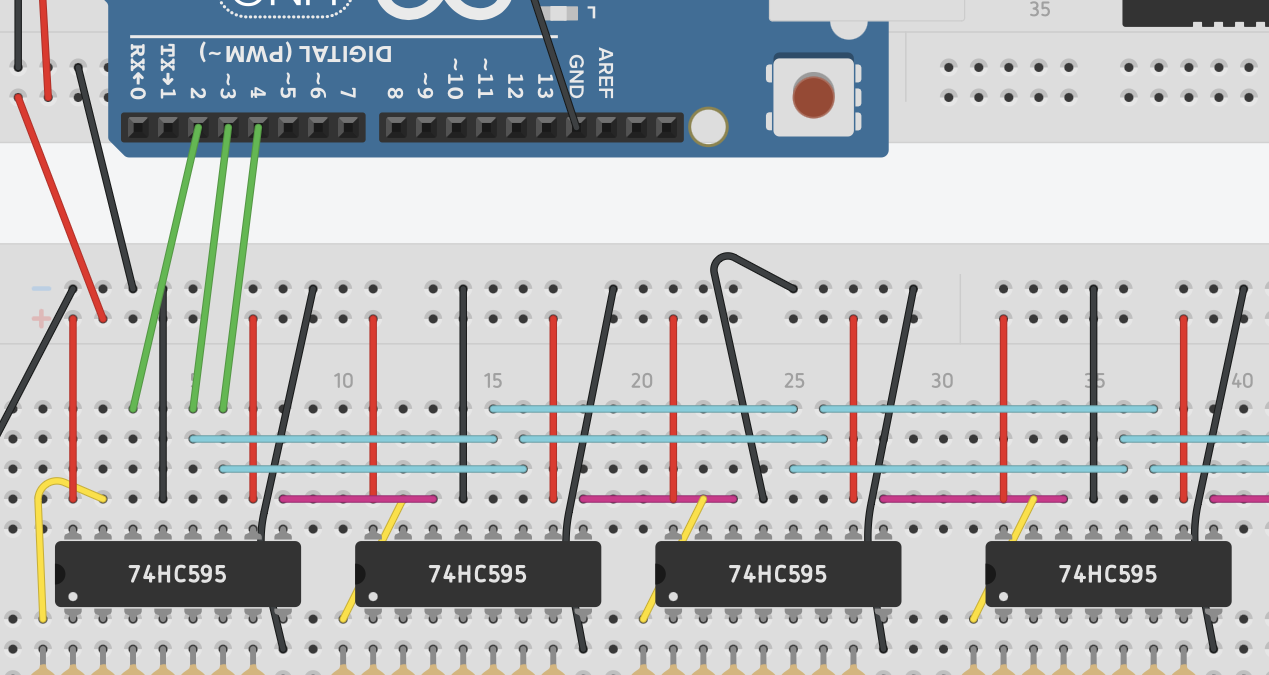
\includegraphics[width=0.9\textwidth]{img/SchaltungSchieberegister}
	\caption{Schaltung der Schieberegister}
	\label{fig:Shifting}
\end{figure}

\subsubsection{MOSFET}

Die Hubmagnete werden jeweils mit 24V und mit bis zu 400mA betrieben.
Um einen hohen Stromfluss zu steuern, können Transistoren verwendet werden.
Für hohe Spannungen und schnelle Schaltvorgänge eigenen sich besonders MOSFETs (Metall-Oxid-Halbleiter-Feldeffekttransistor).
Im Folgenden werden speziell n-MOSFETs verwendet, der mit einem Signal zwischen 0V (leitet nicht) und +5V (voll leitend) angesteuert werden kann.

Der folgende Aufbau ist für die insgesamt 88 Ausgänge der 11 Schieberegister identisch, da jeder Ausgang für die Ansteuerung genau eines Motors zuständig ist.

Der GATE-Pin des MOSFETs erhält das Signal, dass die \enquote{``Durchlässigkeit''} steuert aus einem der Outputs des Schieberegisters.
Der SOURCE-Pin wird mit Ground des gesamten Systems verbunden.
Der DRAIN-Pin wird direkt mit dem entsprechenden Kontakt am Hubmagneten verbunden.

\begin{figure}[htbp]
	\centering
	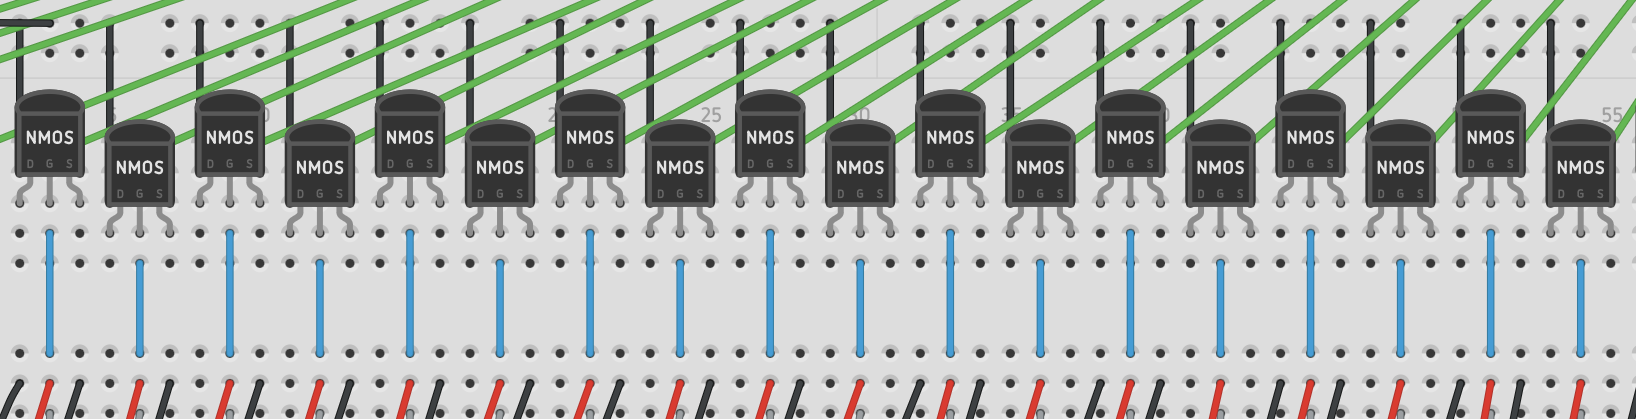
\includegraphics[width=0.9\textwidth]{img/MosSchaltung}
	\caption{Schaltung der Mosfets}
	\label{fig:SchaltungMosfet}
\end{figure}

\subsubsection{Hubmagnet}

Um den Stromkreis zu schließen wird der andere Kontakt des Hubmagnetes mit dem +24V verbunden.
Bei Hubmagneten ist es in der Regel egal, welcher Anschluss an Plus und welcher an Minus angeschlossen wird
(siehe Kapitel \ref{subsec:aktuator}).

\subsubsection{Testen}

Um die Fehlersuche zu erleichtern, werden LEDs in den Schaltplan mit eingebaut.
Diese werden jeweils mit einem entsprechenden $1k\Omega$ Widerstand parallel zu den Motoren angeschlossen.
So kann anhand der Helligkeit der LED die Intensität abgelesen werden, mit der eine Taste gespielt wird.
\newline

Für insgesamt 4 Hubmagnete (Wobei in dem Schema Motoren gewählt wurden, da das Programm keine Hubmagnete als Komponenten
zur Verfügung stellt) und 2 Schieberegister sieht die Darstellung des Schaltplans Schematisch wie folgt aus:

\begin{figure}[htbp]
	\centering
	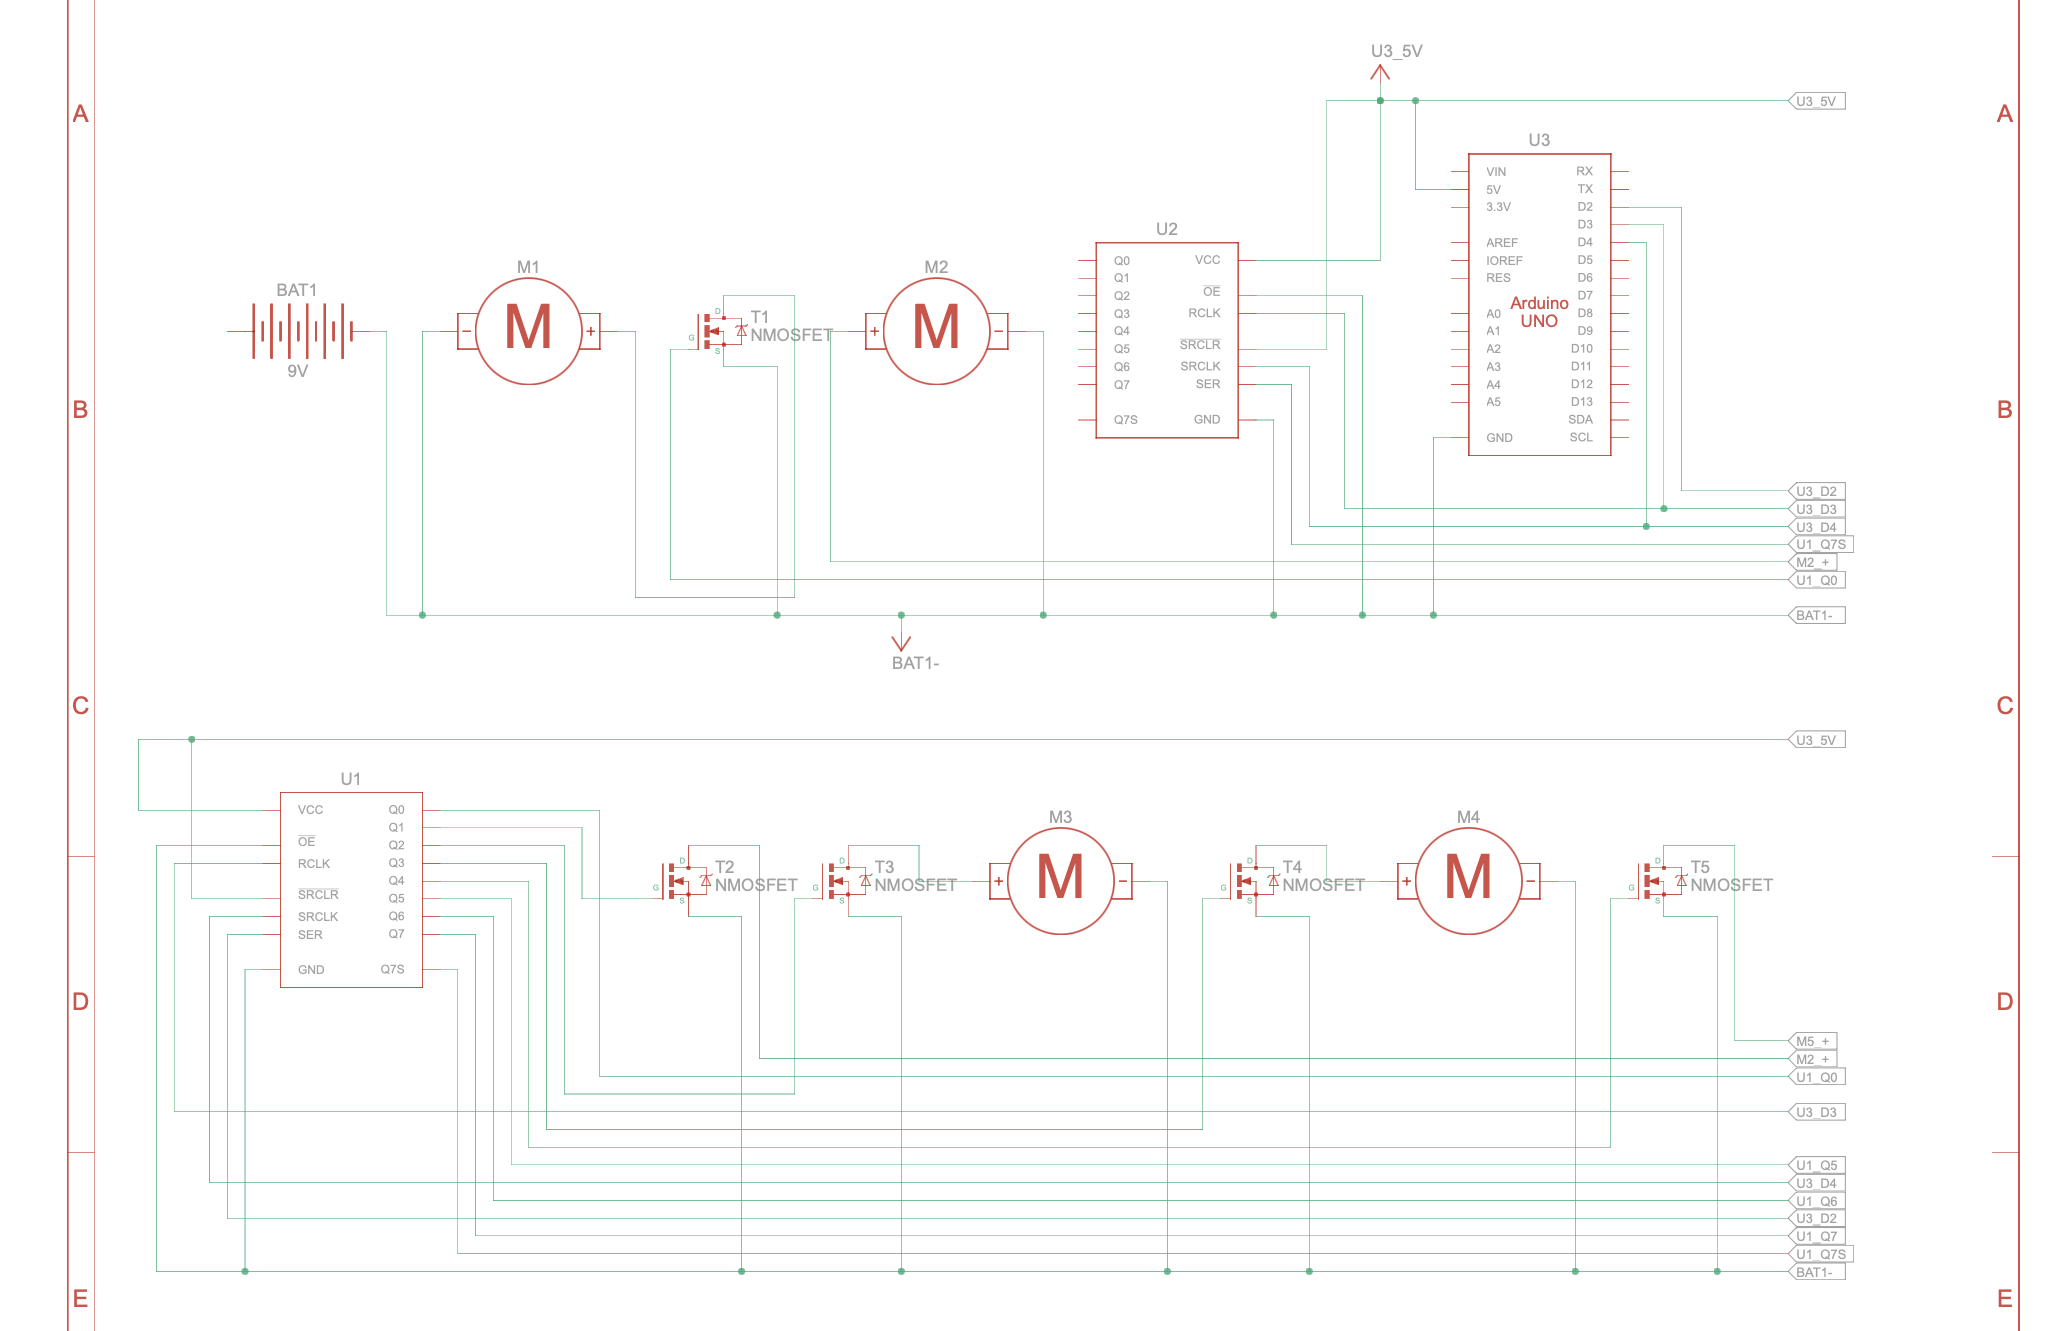
\includegraphics[width=0.9\textwidth]{img/SchematischeSchaltungExp}
	\caption{Beispielhaftes Schema des Schaltplans}
	\label{img:SchaltungExpSchema}
\end{figure}


